\documentclass[preview]{standalone}


\begin{document}

\section{Theorems}
\begin{figure}[!h]
    \centering
    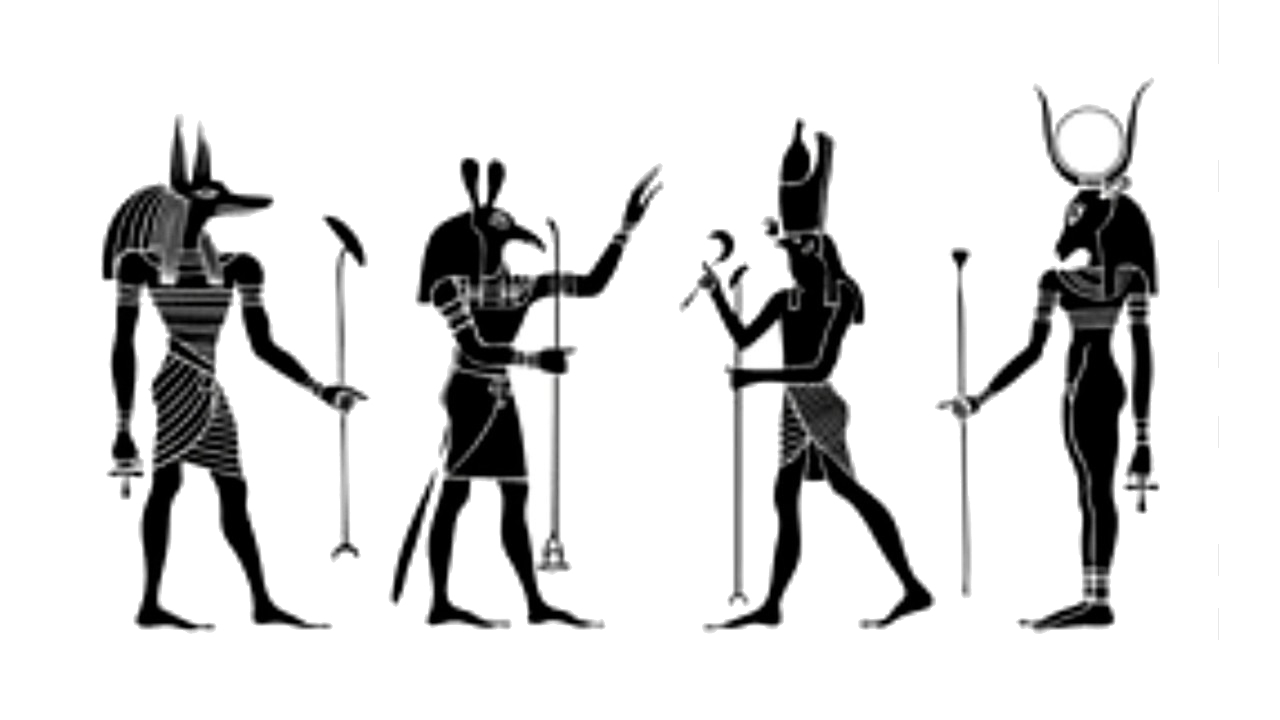
\includegraphics[width=5.75cm]{../resources/jpg/2.2.set.operations/set.jpg}
\end{figure}


% ============================== 0018 Theorem 2205 ================================
\subsection[The set complementation law.]
    {
        \color{section}Theorem 18 \color{black} : the set complementation law.
    }
\documentclass[preview]{standalone}
\usepackage{amssymb, amsthm}
\usepackage{mathtools}
\usepackage{bm}


\newtheorem{theorem}{Theorem}
\renewcommand\qedsymbol{$\blacksquare$}


\begin{document}


\begin{theorem} %[\textbf{2205}] \color{black}
    Let \bm{$\Lambda$} be a subset of \space \bm{$\Omega$}.
    \bm{$\overline{\overline{\Lambda}} = \Lambda$}.
\end{theorem}
\begin{proof} \color{black}
    Suppose there exists an element \bm{$\chi$} such that \bm{$\chi$} is a member of 
    \bm{$\overline{\overline{\Lambda}}$}. 
    By the definition for set complementation, 
    and by the defintion for set membership, 
    that is 
    \begin{equation*}
        \Big \langle \chi \in \overline{\overline{\Lambda}} \Big \rangle 
            \equiv
        \Big \langle \chi \notin \overline{\Lambda} \Big \rangle 
            \equiv
        \lnot \Big \langle \chi \in \overline{\Lambda} \Big \rangle 
            \equiv
        \lnot \Big \langle \chi \notin \Lambda \Big \rangle 
            \equiv
        \lnot \Big \langle \lnot \big \langle \chi \in \Lambda \big \rangle \Big \rangle
    \end{equation*}
    By the logical law of double negation, $\bm{\chi \in \Lambda}$.
    Since logical equivalence is biconditional by definition, 
    this sequence of equivalencies proves both, that 
    \begin{equation*}
        \Big \langle 
            \overline{\overline{\Lambda}}
                \subseteq 
            \Lambda
        \Big \rangle 
            \land 
        \Big \langle 
            \Lambda
                \subseteq 
            \overline{\overline{\Lambda}}
        \Big \rangle
    \end{equation*}
    $\therefore \text{\space} \bm{\overline{\overline{\Lambda}} = \Lambda$}; 
    the complementation law for sets.
\end{proof}


\end{document}
\pagebreak


% ============================= 0019 Theorem 2206a ================================
\subsection[The identity law for set union.]
    {
        \color{section}Theorem 19 \color{black} : the identity law for set union.
    }
\documentclass[preview]{standalone}
\usepackage{amssymb, amsthm}
\usepackage{mathtools}
\usepackage{bm}


\newtheorem{theorem}{Theorem}
\renewcommand\qedsymbol{$\blacksquare$}


\begin{document}


\begin{theorem} %[\textbf{2206a}]
    Let \bm{$\Xi$} be a set. 
    The set identity for \bm{$\Xi$} is \bm{$\Xi \cup \varnothing = \Xi$}.
\end{theorem}
\begin{proof}
    Suppose there exists an element \bm{$\zeta$} such that \bm{$\zeta$} is a member of 
    \bm{$\Xi \cup \varnothing$}. 
    By the definition of set union, that is 
    \begin{equation*}
        \Big \langle \zeta \in \Xi \Big \rangle 
            \lor 
        \Big \langle \zeta \in \varnothing \Big \rangle
    \end{equation*}
    The logical identity for the statement \bm{$\zeta \in \varnothing$} is trivially \bm{$\bot$}, 
    because the empty set contains no members. 
    Thus, by that identity, and by the identity law for logical disjunction,
    \begin{equation*} 
        \Bigg\{
            \Big \langle \zeta \in \Xi \Big \rangle 
                \lor 
            \Big \langle \zeta \in \varnothing \Big \rangle
        \Bigg\} 
            \equiv
        \Bigg\{
            \Big \langle \zeta \in \Xi \Big \rangle 
                \lor
            \Big \langle \bot \Big \rangle 
                \equiv
            \Big \langle \zeta \in \Xi \Big \rangle
        \Bigg\}
            \equiv
    \end{equation*}
    \begin{equation*} 
        \Bigg\{
            \Big \langle \zeta \in \Xi \Big \rangle 
                \lor 
            \Big \langle \zeta \in \varnothing \Big \rangle
                \equiv
            \Big \langle \zeta \in \Xi \Big \rangle
        \Bigg\}
    \end{equation*}
    $\therefore$ 
    by the definition for set union,
    the set identity for \bm{$\Xi$} is \bm{$\Xi \cup \varnothing = \Xi$}.
\end{proof}


\end{document}
\sep


% ============================= 0020 Theorem 2206b ================================
\subsection[The identity law for set intersection.]
    {
        \color{section}Theorem 20 \color{black} : the identity law for set intersection.
    }
\documentclass[preview]{standalone}
\usepackage{amssymb, amsthm}
\usepackage{mathtools}
\usepackage{bm}


\newtheorem*{theorem*}{Theorem}
\renewcommand\qedsymbol{$\blacksquare$}


\begin{document}


\begin{theorem} %[\textbf{2206b}]
    Let \bm{$\Xi$} be a set with universal set \bm{$\Omega$}. 
    The set identity for \bm{$\Xi$} is \bm{$\Xi \cap \Omega = \Xi$}.
\end{theorem}
\begin{proof}
    Suppose there exists an element \bm{$\zeta$} such that \bm{$\zeta$} is a member of \bm{$\Xi \cap \Omega$}. 
    By the definition for set intersection, that is
    \begin{equation*}
        \Big \langle \zeta \in \Xi \Big \rangle 
            \land 
        \Big \langle \zeta \in \Omega \Big \rangle
    \end{equation*}
    The logical identity for the statement \bm{$\zeta \in \Omega$} is trivially \bm{$\top$}, 
    because \bm{$\Omega$} is the universe. 
    Thus, by that identity, and by the identity law for logical conjunction, 
    \begin{equation*}
        \Bigg\{
            \Big \langle \zeta \in \Xi \Big \rangle 
                \land 
            \Big \langle \zeta \in \Omega \Big \rangle 
        \Bigg\} 
            \equiv
        \Bigg\{
            \Big \langle \zeta \in \Xi \Big \rangle 
                \land 
            \Big \langle \top \Big \rangle 
                \equiv 
            \Big \langle \zeta \in \Xi \Big \rangle
        \Bigg\}
            \equiv
    \end{equation*}
    \begin{equation*}
        \Bigg\{
            \Big \langle \zeta \in \Xi \Big \rangle 
                \land 
            \Big \langle \zeta \in \Omega \Big \rangle
                \equiv
            \Big \langle \zeta \in \Xi \Big \rangle
        \Bigg\}
    \end{equation*}
    $\therefore$ by the definition for the intersection of sets,
    the set identity for \bm{$\Xi$} is \bm{$\Xi \cap \Omega = \Xi$}.
\end{proof}


\end{document}
\pagebreak


% ============================= 0021 Theorem 2207a ================================
\subsection[Domination for set union.]
    {
        \color{section}Theorem 21 \color{black} : domination for set union.
    }
\documentclass[preview]{standalone}
\usepackage{amssymb, amsthm}
\usepackage{mathtools}
\usepackage{bm}


\newtheorem{theorem}{Theorem}
\renewcommand\qedsymbol{$\blacksquare$}


\begin{document}


\begin{theorem} %[\textbf{2207a}]
    Let \bm{$\Xi$} be a set with universal set \bm{$\Omega$}. 
    \bm{$\Omega$} dominates set union such that 
    \begin{equation*}
        \bm{\Xi \cup \Omega = \Omega}    
    \end{equation*}
\end{theorem}
\begin{proof}
    Suppose there exists an element \bm{$\zeta$} such that \bm{$\zeta$} is a member of 
    \bm{$\Xi \cup \Omega$}. 
    By the definition for set union, that is
    \begin{equation*}
        \Big \langle \zeta \in \Xi \Big \rangle
            \lor 
        \Big \langle \zeta \in \Omega \Big \rangle
    \end{equation*}
    The logical identity for the statement \bm{$\zeta \in \Omega$} is trivially \bm{$\top$}, 
    since \bm{$\Omega$} is the universe. 
    Thus, 
    by that identity, 
    and by the domination law for logical disjunction,
    \begin{equation*}
        \Bigg\{
            \Big \langle \zeta \in \Xi \Big \rangle 
                \lor 
            \Big \langle \zeta \in \Omega \Big \rangle
        \Bigg\}
            \equiv
        \Bigg\{
            \Big \langle \zeta \in \Xi \Big \rangle 
                \lor 
            \Big \langle \top \Big \rangle
                \equiv
            \Big \langle \zeta \in \Omega \Big \rangle
        \Bigg\}
            \equiv
    \end{equation*}
    \begin{equation*}
        \Bigg\{
            \Big \langle \zeta \in \Xi \Big \rangle 
                \lor 
            \Big \langle \zeta \in \Omega \Big \rangle
                \equiv
            \Big \langle \zeta \in \Omega \Big \rangle
        \Bigg\}
    \end{equation*}
    $\therefore$ by the definition for the union of sets, 
    \bm{$\Omega$} dominates set union such that 
    \bm{$\Xi \cup \Omega = \Omega$}.
\end{proof}


\end{document}
\sep
\begin{figure}[!h]
    \centering
    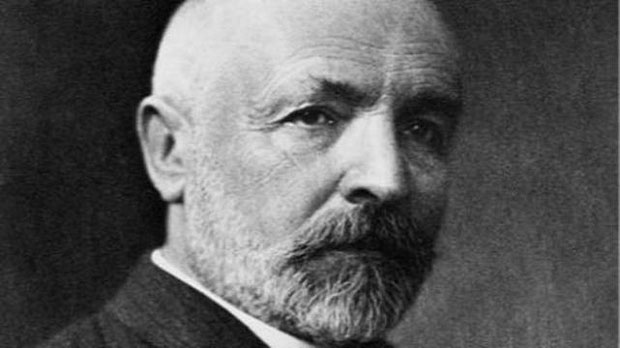
\includegraphics[width=13.75cm]{../resources/jpg/2.2.set.operations/georg_cantor.jpg}
    \caption*{Georg Cantor.}
\end{figure}
\pagebreak


% ============================= 0022 Theorem 2207b ================================
\subsection[Domination for set intersection.]
    {
        \color{section}Theorem 22 \color{black} : domination for set intersection.
    }
\documentclass[preview]{standalone}
\usepackage{amssymb, amsthm}
\usepackage{mathtools}
\usepackage{bm}


\newtheorem{theorem}{Theorem}
\renewcommand\qedsymbol{$\blacksquare$}


\begin{document}


\begin{theorem} %[\textbf{2207b}]
    Let \bm{$\Xi$} be a set. 
    The empty set dominates set intersection such that
    \begin{equation*}
        \bm{\Xi \cap \varnothing = \varnothing}
    \end{equation*}
\end{theorem}
\begin{proof}
    Let \bm{$\zeta$} be an element in \bm{$\Xi \cap \varnothing$}. 
    By the definition for set intersection, that is 
    \begin{equation*}
        \Big \langle \zeta \in \Xi \Big \rangle 
            \land 
        \Big \langle \zeta \in \varnothing \Big \rangle
    \end{equation*}
    The logical identity for the statement \bm{$\zeta \in \varnothing$} is trivially \bm{$\bot$}, 
    since the empty set contains no members. 
    Thus, by that identity, 
    and by the domination law for logical conjunction,
    \begin{equation*}
        \Bigg\{
            \Big \langle \zeta \in \Xi \Big \rangle 
                \land 
            \Big \langle \zeta \in \varnothing \Big \rangle
        \Bigg\}
            \equiv
        \Bigg\{
            \Big \langle \zeta \in \Xi \Big \rangle 
                \land 
            \Big \langle \bot \Big \rangle
                \equiv
            \Big \langle \zeta \in \varnothing \Big \rangle
        \Bigg\}
            \equiv
    \end{equation*}
    \begin{equation*}
        \Bigg\{
            \Big \langle \zeta \in \Xi \Big \rangle 
                \land 
            \Big \langle \zeta \in \varnothing \Big \rangle
                \equiv
            \Big \langle \zeta \in \varnothing \Big \rangle
        \Bigg\}
    \end{equation*}
    $\therefore$ by the definition for the intersection of sets,
    the empty set dominates set intersection such that 
    \bm{$\Xi \cap \varnothing = \varnothing$}.
\end{proof}


\end{document}
\vspace{3\baselineskip}
\begin{figure}[!h]
    \centering
    
\includegraphics[width=6cm]{../resources/jpg/2.2.set.operations/border1.jpg}
\end{figure}
\vspace{2\baselineskip}


% ============================= 0023 Theorem 2208a ================================
\subsection[Idempotence for the union of sets.]
    {
        \color{section}Theorem 23 \color{black} : idempotence for the union of sets.
    }
\documentclass[preview]{standalone}
\usepackage{amssymb, amsthm}
\usepackage{mathtools}
\usepackage{bm}


\newtheorem{theorem}{Theorem}
\renewcommand\qedsymbol{$\blacksquare$}


\begin{document}


\begin{theorem} %[\textbf{2208a}]
    Let \bm{$\Lambda$} be a set. 
    \bm{$\Lambda$} is idempotent such that 
    \bm{$\Lambda \cup \Lambda = \Lambda$}.
\end{theorem}
\begin{proof}
    Let \bm{$\mu$} be an element in \bm{$\Lambda \cup \Lambda$}. 
    By the definition of set union, that is 
    \begin{equation*}
        \Big \langle \mu \in \Lambda \Big \rangle 
            \lor 
        \Big \langle \mu \in \Lambda \Big \rangle
    \end{equation*}
    Thus, by the idempotent law for logical disjunction, 
    \begin{equation*}
        \Big \langle \mu \in \Lambda \Big \rangle 
            \lor 
        \Big \langle \mu \in \Lambda \Big \rangle 
            \equiv 
        \Big \langle \mu \in \Lambda \Big \rangle
    \end{equation*}
    $\therefore$ by the defintion for set union,
    \bm{$\Lambda$} is idempotent such that 
    \bm{$\Lambda \cup \Lambda = \Lambda$}.
\end{proof}


\end{document}
\pagebreak


% ============================= 0024 Theorem 2208b ================================
\subsection[Idempotence for the intersection of sets.]
    {
        \color{section}Theorem 24 \color{black} : idempotence for the intersection of sets.
    }
\documentclass[preview]{standalone}
\usepackage{amssymb, amsthm}
\usepackage{mathtools}
\usepackage{bm}


\newtheorem{theorem}{Theorem}
\renewcommand\qedsymbol{$\blacksquare$}


\begin{document}


\begin{theorem} %[\textbf{2208b}]
    Let \bm{$\Lambda$} be a set.
    \bm{$\Lambda$} is idempotent such that 
    \bm{$\Lambda \cap \Lambda = \Lambda$}.
\end{theorem}
\begin{proof}
    Let \bm{$\mu$} be an element in \bm{$\Lambda \cap \Lambda$}. 
    By the definition for set intersection,
    \begin{equation*}
        \Big \langle \mu \in \Lambda \Big \rangle 
            \land 
        \Big \langle \mu \in \Lambda \Big \rangle
    \end{equation*}
    Thus, by the idempotent law for logical conjunction,
    \begin{equation*}
        \Big \langle \mu \in \Lambda \Big \rangle 
            \land 
        \Big \langle \mu \in \Lambda \big \rangle 
            \equiv 
        \Big \langle \mu \in \Lambda \Big \rangle
    \end{equation*}
    $\therefore$ by the definition for the intersection of sets,
    \bm{$\Lambda$} is idempotent such that 
    \bm{$\Lambda \cap \Lambda = \Lambda$}.
\end{proof}


\end{document}
\sep


% ============================= 0025 Theorem 2209a ================================
\subsection[The complement law for set union.]
    {
        \color{section}Theorem 25 \color{black} : the complement law for set union.
    }
\documentclass[preview]{standalone}
\usepackage{amssymb, amsthm}
\usepackage{mathtools}
\usepackage{bm}


\newtheorem{theorem}{Theorem}
\renewcommand\qedsymbol{$\blacksquare$}


\begin{document}


\begin{theorem}[\textbf{2209a}]
    Let \bm{$\Psi$} be a set with universal set \bm{$\Omega$}.
    \bm{$\Psi \cup \overline{\Psi} = \Omega$}.
\end{theorem}
\begin{proof}
    Let \bm{$\sigma$} be an element in \bm{$\Psi \cup \overline{\Psi}$}. 
    By the definition for set union,  
    \begin{equation*}
        \Big \langle \sigma \in \Psi \Big \rangle 
            \lor 
        \Big \langle \sigma \in \overline{\Psi} \Big \rangle
    \end{equation*}
    The right-hand side of this disjunction is equivalent to \bm{$\sigma \in \Omega - \Psi$}, 
    by the definition for set complementation. 
    By Theorem 45, \bm{$\sigma \in \Omega \cap \overline{\Psi}$}, 
    which is defined as 
    \bm{$\big \langle \sigma \in \Omega \big \rangle 
        \land 
    \big \langle \sigma \notin \Psi \big \rangle$},
    by the definitions for set intersection and set complementation. 
    Thus, the original disjunction is the same as 
    \begin{equation*}
        \Big \langle \sigma \in \Psi \Big \rangle 
            \lor 
        \Bigg[
            \Big \langle \sigma \in \Omega \Big \rangle 
                \land 
            \Big \langle \sigma \notin \Psi \Big \rangle
        \Bigg]
    \end{equation*}
    We must distribute the left-hand side of this disjunction over the conjunction occurring in the right-hand side. 
    We get 
    \begin{equation*}
        \Bigg[
            \Big \langle \sigma \in \Psi \Big \rangle 
                \lor 
            \Big \langle \sigma \in \Omega \Big \rangle
        \Bigg] 
            \land 
        \Bigg[
            \Big \langle \sigma \in \Psi \Big \rangle 
                \lor 
            \Big \langle \sigma \notin \Psi \Big \rangle
        \Bigg]
    \end{equation*}
    By the logical law of negation, 
    the identity for the right-hand side of this conjunction is \bm{$\top$}. 
    The left-hand side of this conjunction is dominated by \bm{$\Omega$}, 
    according to Theorem 21. 
    Therefore, 
    the statement \bm{$\sigma \in \Psi \cup \overline{\Psi}$} can be equivalently stated as 
    \bm{$\big \langle \sigma \in \Omega \big \rangle \land \top$}; 
    the logical identity for which is \bm{$\sigma \in \Omega$}. 
    The converse trivially follows from the fact of logical equivalence. 
    Thus, 
    proves the set complement law for the union of sets, 
    \bm{$\Psi \cup \overline{\Psi} = \Omega$}.
\end{proof}


\end{document}
\pagebreak


% ============================= 0026 Theorem 2209b ================================
\subsection[The complement law for set intersection.]
    {
        \color{section}Theorem 26 \color{black} : the complement law for set intersection.
    }
\documentclass[preview]{standalone}
\usepackage{amssymb, amsthm}
\usepackage{mathtools}
\usepackage{bm}


\newtheorem{theorem}{Theorem}
\renewcommand\qedsymbol{$\blacksquare$}


\begin{document}


\begin{theorem}[\textbf{2209b}]
    Let \bm{$\Xi$} be a set. 
    \bm{$\Xi \cap \overline{\Xi} = \varnothing$}.
\end{theorem}
\begin{proof}
    Let \bm{$\zeta$} be an element in \bm{$\Xi \cap \overline{\Xi}$}. 
    By the definition for the intersection of sets, that is
    \begin{equation*}
        \Big \langle \zeta \in \Xi \Big \rangle 
            \land 
        \Big \langle \zeta \in \overline{\Xi} \Big \rangle
    \end{equation*} 
    According to the definitions for set complementation and set membership, 
    and by the negation law of logic, that is
    \begin{equation*}
        \Bigg\{
            \Big \langle \zeta \in \Xi \Big \rangle 
                \land 
            \Big \langle \zeta \in \overline{\Xi} \Big \rangle
        \Bigg\}
            \equiv
        \Bigg\{
            \Big \langle \zeta \in \Xi \Big \rangle 
                \land 
            \lnot \Big \langle \zeta \in \Xi \Big \rangle
                \equiv
            \Big \langle \bot \Big \rangle
        \Bigg\}
    \end{equation*}
    \bm{$\big \langle \bot \big \rangle$} is trivially the logical identity for 
    the statement \bm{$\zeta \in \varnothing$}, 
    since the empty set contains no members. 
    Thus, 
    by that identity, 
    and following from the series of equivalencies from above,
    \begin{equation*}
        \Big \langle \zeta \in \Xi \Big \rangle 
            \land 
        \Big \langle \zeta \in \overline{\Xi} \Big \rangle 
            \equiv
        \Big \langle \zeta \in \varnothing \Big \rangle
    \end{equation*}
    $\therefore$ the complement law for sets, 
    \bm{$\Xi \cap \overline{\Xi} = \varnothing$}, 
    follows immediately from the definition for the intersection of sets.
\end{proof}


\end{document}
\sep


% ============================= 0027 Theorem 2210a ===============================
\subsection[Subtracting the empty set.]
    {
        \color{section}Theorem 27 \color{black} : subtracting the empty set.
    }
\documentclass[preview]{standalone}
\usepackage{amssymb, amsthm}
\usepackage{mathtools}
\usepackage{bm}


\newtheorem{theorem}{Theorem}
\renewcommand\qedsymbol{$\blacksquare$}


\begin{document}


\begin{theorem}[\textbf{2210a}]
    Let \bm{$\Xi$} be a set. 
    \bm{$\Xi - \varnothing = \Xi$}.
\end{theorem}
\begin{proof}
    Suppose there exists an element \bm{$\zeta$} such that \bm{$\zeta$} is a member of 
    \bm{$\Xi - \varnothing$}.
    By the definition for set difference, that is
    \begin{equation*}
        \Big \langle \zeta \in \Xi \Big \rangle
            \land 
        \Big \langle \zeta \notin \varnothing \Big \rangle
    \end{equation*}
    It is trivial that the logical identity for the statement 
    \bm{$\zeta \notin \varnothing$} is \bm{$\top$},
    since the empty set contains no members. 
    Thus, by that identity, 
    and by the identity law for logical conjunction,
    \begin{equation*}
        \Bigg\{
            \Big \langle \zeta \in \Xi \Big \rangle
                \land 
            \Big \langle \zeta \notin \varnothing \Big \rangle
        \Bigg\}
            \equiv
        \Bigg\{
            \Big \langle \zeta \in \Xi \Big \rangle
                \land 
            \Big \langle \top \Big \rangle
                \equiv
            \Big \langle \zeta \in \Xi \Big \rangle
        \Bigg\}
            \equiv
    \end{equation*}
    \begin{equation*}
        \Bigg\{
            \Big \langle \zeta \in \Xi \Big \rangle
                \land 
            \Big \langle \zeta \notin \varnothing \Big \rangle
                \equiv
            \Big \langle \zeta \in \Xi \Big \rangle
        \Bigg\}
    \end{equation*}
    $\therefore$ by the definition for set difference,
    \bm{$\Xi - \varnothing = \Xi$}.
\end{proof}


\end{document}
\pagebreak


% ============================= 0028 Theorem 2210b ===============================
\subsection[The empty set minus any set is empty.]
    {
        \color{section}Theorem 28 \color{black} : the empty set minus any set is empty.
    }
\documentclass[preview]{standalone}
\usepackage{amssymb, amsthm}
\usepackage{mathtools}
\usepackage{bm}


\newtheorem{theorem}{Theorem}
\renewcommand\qedsymbol{$\blacksquare$}


\begin{document}


\begin{theorem}[\textbf{2210b}]
    Let \bm{$\Xi$} be a set. 
    \bm{$\varnothing - \Xi = \varnothing$}.
\end{theorem}
\begin{proof}
    Let \bm{$\zeta$} be an element in \bm{$\varnothing - \Xi$}. 
    By the definition for set difference,
    \begin{equation*}
        \Big \langle \zeta \in \varnothing \Big \rangle
            \land 
        \Big \langle \zeta \notin \Xi \Big \rangle
    \end{equation*}
    The logical identity for the statement \bm{$\zeta \in \varnothing$} is trivially \bm{$\bot$}, 
    since the empty set contains no members. 
    Thus, by that identity, and by the domination law for logical conjunction,
    \begin{equation*}
        \Bigg\{
            \Big \langle \zeta \in \varnothing \Big \rangle
                \land 
            \Big \langle \zeta \notin \Xi \Big \rangle
        \Bigg\}
            \equiv
        \Bigg\{
            \Big \langle \bot \Big \rangle
                \land 
            \Big \langle \zeta \notin \Xi \Big \rangle 
                \equiv 
            \Big \langle \bot \Big \rangle
        \Bigg\}
            \equiv
    \end{equation*}
    \begin{equation*}
        \Bigg\{
            \Big \langle \zeta \in \varnothing \Big \rangle
                \land 
            \Big \langle \zeta \notin \Xi \Big \rangle
                \equiv
            \Big \langle \zeta \in \varnothing \Big \rangle
        \Bigg\}
    \end{equation*}
    $\therefore$ by the definition for set difference,  
    \bm{$\varnothing - \Xi = \varnothing$}
\end{proof}


\end{document}
\vspace{2.9\baselineskip}
\begin{figure}[!h]
    \centering
    
\includegraphics[width=8cm]{../resources/jpg/2.2.set.operations/border2.jpg}
\end{figure}
\vspace{2\baselineskip}


% ============================= 0029 Theorem 2211a ===============================
\subsection[Set union is commutative.]
    {
        \color{section}Theorem 29 \color{black} : set union is commutative.
    }
\documentclass[preview]{standalone}
\usepackage{amssymb, amsthm}
\usepackage{mathtools}
\usepackage{bm}


\newtheorem{theorem}{Theorem}
\renewcommand\qedsymbol{$\blacksquare$}


\begin{document}


\begin{theorem}[\textbf{2211a}]
    Let \bm{$\mathrm{A}$} and \bm{$\Lambda$} be sets. 
    The union of \bm{$\mathrm{A}$} and \bm{$\Lambda$} is commutative.
\end{theorem}
\begin{proof}
    Let \bm{$\lambda$} be an element in \bm{$\mathrm{A} \cup \Lambda$}. 
    By the definition for set union,
    \begin{equation*}
        \Big \langle \lambda \in \mathrm{A} \Big \rangle 
            \lor 
        \Big \langle \lambda \in \Lambda \Big \rangle
    \end{equation*} 
    Because logical disjunction is commutative, 
    that is 
    \begin{equation*}
        \Bigg[
            \Big \langle \lambda \in \mathrm{A} \Big \rangle
                \lor 
            \Big \langle \lambda \in \Lambda \Big \rangle
        \Bigg]
            \equiv 
        \Bigg[
            \Big \langle \lambda \in \Lambda \Big \rangle
                \lor 
            \Big \langle \lambda \in \mathrm{A} \Big \rangle
        \Bigg]
    \end{equation*} 
    $\therefore \text{\space} 
    \bm{\mathrm{A} \cup \Lambda = \Lambda \cup \mathrm{A}$}, 
    and the union of \bm{$\mathrm{A}$} and \bm{$\Lambda$} is indeed commutative.
\end{proof}


\end{document}
\pagebreak


% ============================= 0030 Theorem 2211b ===============================
\subsection[Set intersection is commutative.]
    {
        \color{section}Theorem 30 \color{black} : set intersection is commutative.
    }
\documentclass[preview]{standalone}
\usepackage{amssymb, amsthm}
\usepackage{mathtools}
\usepackage{bm}


\newtheorem{theorem}{Theorem}
\renewcommand\qedsymbol{$\blacksquare$}


\begin{document}


\begin{theorem}[\textbf{2211b}]
    Let \bm{$\mathrm{A}$} and \bm{$\Lambda$} be sets. 
    The intersection of \bm{$\mathrm{A}$} and \bm{$\Lambda$} is commutative.
\end{theorem}
\begin{proof}
    Let \bm{$\lambda$} be an element in \bm{$\mathrm{A} \cap \Lambda$}. 
    By the definition for set intersection, 
    \begin{equation*}
        \Big \langle \lambda \in \mathrm{A} \Big \rangle 
            \land 
        \Big \langle \lambda \in \Lambda \Big \rangle
    \end{equation*}
    Because logical conjunction is commutative, that is
    \begin{equation*}
        \Bigg[
            \Big \langle \lambda \in \mathrm{A} \Big \rangle 
                \land 
            \Big \langle \lambda \in \Lambda \Big \rangle
        \Bigg]
            \equiv
        \Bigg[
            \Big \langle \lambda \in \Lambda \Big \rangle 
                \land 
            \Big \langle \lambda \in \mathrm{A} \Big \rangle
        \Bigg]
    \end{equation*}
    $\therefore \text{\space} 
    \bm{\mathrm{A} \cap \Lambda = \Lambda \cap \mathrm{A}}$, 
    and indeed the intersection of \bm{$\mathrm{A}$} and \bm{$\Lambda$} is commutative.
\end{proof}


\end{document}
\vspace{2.9\baselineskip}
\begin{figure}[!h]
    \centering
    
\includegraphics[width=7cm]{../resources/jpg/2.2.set.operations/border3.jpg}
\end{figure}
\vspace{2.8\baselineskip}

% ============================= 0031 Theorem 2212 ================================
\subsection[Absorption for union over intersection.]
    {
        \color{section}Theorem 31 \color{black} : absorption for union over intersection.
    }
\documentclass[preview]{standalone}
\usepackage{amssymb, amsthm}
\usepackage{mathtools}
\usepackage{bm}


\newtheorem{theorem}{Theorem}
\renewcommand\qedsymbol{$\blacksquare$}


\begin{document}


\begin{theorem}[\textbf{2212}]
    Let \bm{$\mathrm{A}$} and \bm{$\Lambda$} be sets. 
    \bm{$
    \mathrm{A} 
        \cup 
    \big \langle \mathrm{A} \cap \Lambda \big \rangle 
        = 
    \mathrm{A}$}.
\end{theorem}
\begin{proof}
    Let \bm{$\lambda$} be an element in 
    \bm{$
    \mathrm{A} 
        \cup 
    \big \langle \mathrm{A} \cap \Lambda \big \rangle
    $}. 
    By the definitions for the union of sets and the intersection of sets, that is
    \begin{equation*}
        \Big \langle \lambda \in \mathrm{A} \Big \rangle 
            \lor 
        \bigg[
            \Big \langle \lambda \in \mathrm{A} \Big \rangle 
                \land 
            \Big \langle \lambda \in \Lambda \Big \rangle
        \bigg]
    \end{equation*}
    It follows immediately from the laws of logical absorption that
    \begin{equation*}
        \Bigg\{
            \Big \langle \lambda \in \mathrm{A} \Big \rangle 
                \lor 
            \bigg[
                \Big \langle \lambda \in \mathrm{A} \Big \rangle 
                    \land 
                \Big \langle \lambda \in \Lambda \Big \rangle
            \bigg]
        \Bigg\}
            \equiv 
        \bigg \langle \lambda \in \mathrm{A} \bigg \rangle 
    \end{equation*}
    $\therefore$ by the definitions for set union and set intersection, 
    \bm{$
    \mathrm{A} 
        \cup 
    \big \langle \mathrm{A} \cap \Lambda \big \rangle 
        = 
    \mathrm{A}$}; 
    the absorption law for set union over intersection.
\end{proof}


\end{document}
\pagebreak


% ============================= 0032 Theorem 2213 ================================
\subsection[Absorption for intersection over union.]
    {
        \color{section}Theorem 32 \color{black} : absorption for intersection over union.
    }
\documentclass[preview]{standalone}
\usepackage{amssymb, amsthm}
\usepackage{mathtools}
\usepackage{bm}


\newtheorem{theorem}{Theorem}
\renewcommand\qedsymbol{$\blacksquare$}


\begin{document}


\begin{theorem}[\textbf{2213}]
    Let \bm{$\mathrm{A}$} and \bm{$\Lambda$} be sets. 
    \bm{$
    \mathrm{A} 
        \cap 
    \big \langle \mathrm{A} \cup \Lambda \big \rangle 
        = 
    \mathrm{A}
    $}.
\end{theorem}
\begin{proof}
    Let \bm{$\lambda$} be an element in 
    \bm{$
    \mathrm{A} 
        \cap 
    \big \langle \mathrm{A} \cup \Lambda \big \rangle
    $}. 
    By the definitions for set union and set intersection, that is 
    \begin{equation*}
        \Big \langle \lambda \in \mathrm{A} \Big \rangle 
            \land 
        \bigg[
            \Big \langle \lambda \in \mathrm{A} \Big \rangle 
                \lor 
            \Big \langle \lambda \in \Lambda \Big \rangle
        \bigg]
    \end{equation*}
    It follows immediately from the laws of logical absorption that
    \begin{equation*}
        \Bigg\{
            \Big \langle \lambda \in \mathrm{A} \Big \rangle 
                \land 
            \bigg[
                \Big \langle \lambda \in \mathrm{A} \Big \rangle 
                    \lor 
                \Big \langle \lambda \in \Lambda \Big \rangle
            \bigg]
        \Bigg\}
            \equiv
        \bigg \langle \lambda \in \mathrm{A} \bigg \rangle 
    \end{equation*}
    $\therefore$ by the definitions for set intersection and set union, 
    \bm{$
    \mathrm{A} 
        \cap 
    \big \langle \mathrm{A} \cup \Lambda \big \rangle 
        = 
    \mathrm{A}
    $}; 
    the absorption law for set intersection over union. 
\end{proof}


\end{document}
\vspace{1.1\baselineskip}
\begin{figure}[!h]
    \centering
    
\includegraphics[width=9cm]{../resources/jpg/2.2.set.operations/border4.jpg}
\end{figure}
\vspace{.1\baselineskip}


% ============================= 0033 Theorem 2215 ================================
\subsection[DeMorgan's Law for a complemented union.]
    {
        \color{section}Theorem 33 \color{black} : DeMorgan's for complemented unions.
    }
\documentclass[preview]{standalone}
\usepackage{amssymb, amsthm}
\usepackage{mathtools}
\usepackage{bm}


\newtheorem{theorem}{Theorem}
\renewcommand\qedsymbol{$\blacksquare$}


\begin{document}


\begin{theorem}[\textbf{2215}]
    Let \bm{$\mathrm{A}$} and \bm{$\Lambda$} be sets. 
    \bm{$
    \overline{\mathrm{A} \cup \Lambda} 
        = 
    \overline{\mathrm{A}} \cap \overline{\Lambda}
    $}.
\end{theorem}
\begin{proof}
    Let \bm{$\lambda$} be an element in \bm{$\overline{\mathrm{A} \cup \Lambda}$}. 
    By the definitions for set complementation, and set membership, that is 
    \bm{$\lnot 
            \Big[
                \lambda \in \big \langle \mathrm{A} \cup \Lambda \big \rangle 
            \Big]
    $}. 
    Hence, by the definition of set union, 
    \begin{equation*}
        \lnot \bigg[
            \Big \langle \lambda \in \mathrm{A} \Big \rangle 
                \lor 
            \Big \langle \lambda \in \Lambda \Big \rangle
        \bigg]    
    \end{equation*}
    By DeMorgans law (from logic), 
    and by the definitions for set complementation
    and set membership
    \begin{equation*}
        \Bigg\{
            \lnot \bigg[
                \Big \langle \lambda \in \mathrm{A} \Big \rangle 
                    \lor 
                \Big \langle \lambda \in \Lambda \Big \rangle
            \bigg]
        \Bigg\}
        \equiv
        \Bigg\{
            \lnot \Big \langle \lambda \in \mathrm{A} \Big \rangle 
                \land 
            \lnot \Big \langle \lambda \in \Lambda \Big \rangle
        \Bigg\}
        \equiv
    \end{equation*}
    \begin{equation*}
        \Bigg\{
            \Big \langle \lambda \in \overline{\mathrm{A}} \Big \rangle 
                \land 
            \Big \langle \lambda \in \overline{\Lambda} \Big \rangle
        \Bigg\}
    \end{equation*}
    $\therefore$ by the definition of set intersection,
    \bm{$
    \overline{\mathrm{A} \cup \Lambda} 
        = 
    \overline{\mathrm{A}} \cap \overline{\Lambda}
    $};
    DeMorgans law for sets.
\end{proof}


\end{document}
\pagebreak


% ============================= 0034 Theorem 2216a ===============================
\subsection[Intersection is a subset of its operands.]
    {
        \color{section}Theorem 34 \color{black} : intersection is a subset of its operands.
    }
\documentclass[preview]{standalone}
\usepackage{amssymb, amsthm}
\usepackage{mathtools}
\usepackage{bm}


\newtheorem{theorem}{Theorem}
\renewcommand\qedsymbol{$\blacksquare$}


\begin{document}


\begin{theorem}[\textbf{2216a}]
    Let \bm{$\mathrm{A}$} and \bm{$\Lambda$} be sets. 
    \bm{$
    \big \langle \mathrm{A} \cap \Lambda \big \rangle 
        \subseteq 
    \mathrm{A}
    $}.
\end{theorem}
\begin{proof}
    Let \bm{$\lambda$} be an element in \bm{$\mathrm{A} \cap \Lambda$}. 
    By the definition for set intersection,
    \begin{equation*}
        \Big \langle \lambda \in \mathrm{A} \Big \rangle 
            \land 
        \Big \langle \lambda \in \Lambda \Big \rangle   
    \end{equation*}
    It trivially follows from the simplification rule of inference that 
    \begin{equation*}
        \bigg[
            \Big \langle \lambda \in \mathrm{A} \Big \rangle 
                \land 
            \Big \langle \lambda \in \Lambda \Big \rangle
        \bigg]
            \rightarrow
        \Big \langle \lambda \in \mathrm{A} \Big \rangle
    \end{equation*}
    $\therefore$ 
    \bm{$
    \big \langle \mathrm{A} \cap \Lambda \big \rangle 
        \subseteq 
    \mathrm{A}
    $}, by the definition of subsets.
\end{proof}


\end{document}
\vspace{2\baselineskip}
\begin{figure}[!h]
    \centering
    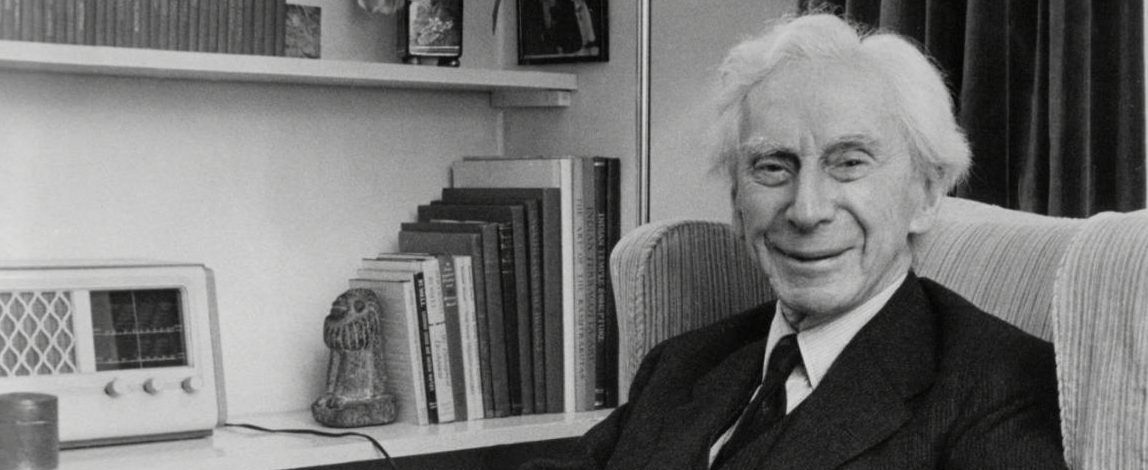
\includegraphics[width=14cm]{../resources/jpg/2.2.set.operations/russel.jpg}
    \caption*{Bertrand Russel.}
\end{figure}


% ============================= 0035 Theorem 2216b ===============================
\subsection[A set is a subset of its union.]
    {
        \color{section}Theorem 35 \color{black} : a set is a subset of its union.
    }
\documentclass[preview]{standalone}
\usepackage{amssymb, amsthm}
\usepackage{mathtools}
\usepackage{bm}


\newtheorem{theorem}{Theorem}
\renewcommand\qedsymbol{$\blacksquare$}


\begin{document}


\begin{theorem}[\textbf{2216b}]
    Let \bm{$\mathrm{A}$} and \bm{$\Lambda$} be sets. 
    \bm{$
    \mathrm{A} 
        \subseteq 
    \big \langle \mathrm{A} \cup \Lambda \big \rangle
    $}.
\end{theorem}
\begin{proof}
    Suppose there existed and element \bm{$\lambda$} such that 
    \bm{$\lambda$} were a member of \bm{$\mathrm{A}$}.
    It follows from the addition rule of inference that
    \begin{equation*}
        \Big \langle \lambda \in \mathrm{A} \Big \rangle
            \rightarrow
        \bigg[ 
            \Big \langle \lambda \in \mathrm{A} \Big \rangle
                \lor 
            \Big \langle \lambda \in \Lambda \Big \rangle
        \bigg]
    \end{equation*}
    $\therefore$ by the definitons for set union and subsets,
    \bm{$
    \mathrm{A} 
        \subseteq 
    \big \langle \mathrm{A} \cup \Lambda \big \rangle
    $}.
\end{proof}


\end{document}
\pagebreak


% ============================= 0036 Theorem 2216c ===============================
\subsection[Set difference is a subset of its left-hand side.]
    {
        \color{section}Theorem 36 \color{black} : difference is a subset of its left side.
    }
\documentclass[preview]{standalone}
\usepackage{amssymb, amsthm}
\usepackage{mathtools}
\usepackage{bm}


\newtheorem{theorem}{Theorem}
\renewcommand\qedsymbol{$\blacksquare$}


\begin{document}


\begin{theorem}[\textbf{2216c}]
    Let \bm{$\mathrm{A}$} and \bm{$\Lambda$} be sets. 
    \bm{$
    \big \langle \mathrm{A} - \Lambda \big \rangle 
        \subseteq 
    \mathrm{A}
    $}.
\end{theorem}
\begin{proof}
    Let \bm{$\lambda$} be an element in \bm{$\mathrm{A} - \Lambda$}. 
    By the definition for set difference,
    \begin{equation*}
        \Big \langle \lambda \in \mathrm{A} \Big \rangle
            \land
        \Big \langle \lambda \notin \Lambda \Big \rangle   
    \end{equation*}
    It trivially follows from the simplification rule of inference that
    \begin{equation*}
        \bigg[
            \Big \langle \lambda \in \mathrm{A} \Big \rangle
                \land
            \Big \langle \lambda \notin \Lambda \Big \rangle
        \bigg]
            \rightarrow
        \Big \langle \lambda \in \mathrm{A} \Big \rangle
    \end{equation*}
    $\therefore$ 
    \bm{$
    \big \langle \mathrm{A} - \Lambda \big \rangle 
        \subseteq 
    \mathrm{A}
    $},
    by the definition for subsets.
\end{proof}


\end{document}
\vspace{1.5\baselineskip}
\begin{figure}[!h]
    \centering
    
\includegraphics[width=8cm]{../resources/jpg/2.2.set.operations/border5.jpg}
\end{figure}
\vspace{1\baselineskip}


% ============================= 0037 Theorem 2216d ===============================
\subsection[Alpha intersect lambda minus alpha is empty.]
    {
        \color{section}Theorem 37 \color{black} : alpha intersect lambda minus alpha.
    }
\documentclass[preview]{standalone}
\usepackage{amssymb, amsthm}
\usepackage{mathtools}
\usepackage{bm}


\newtheorem{theorem}{Theorem}
\renewcommand\qedsymbol{$\blacksquare$}


\begin{document}


\begin{theorem}[\textbf{2216d}]
    Let \bm{$\mathrm{A}$} and \bm{$\Lambda$} be sets. 
    \bm{$
    \mathrm{A} 
        \cap 
    \big \langle \Lambda - \mathrm{A} \big \rangle 
        = 
    \varnothing
    $}.
\end{theorem}
\begin{proof}
    Let \bm{$\lambda$} be an element in 
    \bm{$\mathrm{A} \cap \big \langle \Lambda - \mathrm{A} \big \rangle$}. 
    By the definitions for set difference, 
    and set intersection, that is
    \begin{equation*}
       \Big \langle \lambda \in \mathrm{A} \Big \rangle
            \land
        \bigg[
            \Big \langle \lambda \in \Lambda \Big \rangle
                \land
            \Big \langle \lambda \notin \mathrm{A} \Big \rangle
        \bigg] 
    \end{equation*}
    Since logical conjunction is associative, 
    the logical identity for this statement is \bm{$\bot$}, 
    by the negation law for logical conjunction, 
    and by the domination law for logical conjunction. 
    It is trivial that the logical identity for the statement
    \bm{$\lambda \in \varnothing$} is \bm{$\bot$}, 
    since the empty set contains no members. 
    Thus,
    \begin{equation*}
        \Big \langle \lambda \in \mathrm{A} \Big \rangle
             \land
         \bigg[
             \Big \langle \lambda \in \Lambda \Big \rangle
                 \land
             \Big \langle \lambda \notin \mathrm{A} \Big \rangle
         \bigg] 
            \equiv
        \Big \langle \lambda \in \varnothing \Big \rangle
     \end{equation*}
    $\therefore$ 
    by the definitions for set difference and intersection,
    \bm{$
    \mathrm{A} 
        \cap 
    \big \langle \Lambda - \mathrm{A} \big \rangle 
        = 
    \varnothing
    $}.
\end{proof}


\end{document}
\sep
\pagebreak


% ============================= 0038 Theorem 2216e ===============================
\subsection[Alpha union lambda minus alpha.]
    {
        \color{section}Theorem 38 \color{black} : alpha union lambda minus alpha.
    }
\documentclass[preview]{standalone}
\usepackage{amssymb, amsthm}
\usepackage{mathtools}
\usepackage{bm}


\newtheorem{theorem}{Theorem}
\renewcommand\qedsymbol{$\blacksquare$}


\begin{document}


\begin{theorem}[\textbf{2216e}]
    Let \bm{$\mathrm{A}$} and \bm{$\Lambda$} be sets. 
    \bm{$
    \mathrm{A} 
        \cup 
    \big \langle \Lambda - \mathrm{A} \big \rangle 
        = 
    \mathrm{A} \cup \Lambda
    $}.
\end{theorem}
\begin{proof}
    Let \bm{$\lambda$} be an element in 
    \bm{$\mathrm{A} \cup \big \langle \Lambda - \mathrm{A} \big \rangle$}. 
    By the definitions for set difference, and set union, that is
    \begin{equation*}
        \Big \langle \lambda \in \mathrm{A} \Big \rangle 
            \lor 
        \bigg[
            \Big \langle \lambda \in \Lambda \Big \rangle 
                \land 
            \Big \langle \lambda \notin \mathrm{A} \Big \rangle 
        \bigg] 
    \end{equation*}
    Distributing the logical disjunction over logical conjunction yields
    \begin{equation*}
        \bigg[
            \Big \langle \lambda \in \mathrm{A} \Big \rangle 
                \lor 
            \Big \langle \lambda \in \Lambda \Big \rangle
        \bigg]
            \land
        \bigg[
            \Big \langle \lambda \in \mathrm{A} \Big \rangle
                \lor
            \Big \langle \lambda \notin \mathrm{A} \Big \rangle 
        \bigg]
    \end{equation*} 
    By the negation law for logical disjunction, 
    and by the identity law for logical conjunction, that is
    \begin{equation*}
        \Big \langle \lambda \in \mathrm{A} \Big \rangle 
        \lor 
        \Big \langle \lambda \in \Lambda \Big \rangle
    \end{equation*}
    Thus, 
    \begin{equation*}
        \Big \langle \lambda \in \mathrm{A} \Big \rangle 
            \lor 
        \bigg[
            \Big \langle \lambda \in \Lambda \Big \rangle 
                \land 
            \Big \langle \lambda \notin \mathrm{A} \Big \rangle 
        \bigg]
        \equiv
        \Big \langle \lambda \in \mathrm{A} \Big \rangle 
            \lor 
        \Big \langle \lambda \in \Lambda \Big \rangle\
    \end{equation*}
    $\therefore$ by the definition of set union,
    \bm{$
    \mathrm{A} 
        \cup 
    \big \langle \Lambda - \mathrm{A} \big \rangle 
        = 
    \mathrm{A} \cup \Lambda
    $}.
\end{proof}


\end{document}
\sep


% ============================= 0039 Theorem 2217 ================================
\subsection[DeMorgan's law for a union of complements.]
    {
        \color{section}Theorem 39 \color{black} : DeMorgan's for a union of complements.
    }
\documentclass[preview]{standalone}
\usepackage{amssymb, amsthm}
\usepackage{mathtools}
\usepackage{bm}


\newtheorem{theorem}{Theorem}
\renewcommand\qedsymbol{$\blacksquare$}


\begin{document}


\begin{theorem}[\textbf{2217}]
    Let \bm{$\mathrm{A}$}, \bm{$\Lambda$}, and \bm{$\Delta$} be sets. 
    \bm{$
    \overline{
            \mathrm{A} 
                \cap 
            \Lambda 
                \cap 
            \Delta
    } 
        = 
    \overline{\mathrm{A}} 
        \cup 
    \overline{\Lambda} 
        \cup 
    \overline {\Delta}
    $}.
\end{theorem}
\begin{proof} \color{black}
    Let \bm{$\lambda$} be an element in 
    \bm{$\overline{\mathrm{A} \cap \Lambda \cap \Delta}$}. 
    By the definitions for set complementation and set membership, that is
    \begin{equation*}
        \lambda \notin \mathrm{A} \cap \Lambda \cap \Delta 
            \equiv 
        \lnot \big[ \lambda \in
            \mathrm{A} \cap \Lambda \cap \Delta
        \big]
    \end{equation*}
    The following statement is equivalent, by the definition for set intersection,
    \begin{equation*}
        \lnot \Big[
            \big \langle \lambda \in \mathrm{A} \big \rangle 
                \land 
            \big \langle \lambda \in \Lambda \big \rangle
                \land 
            \big \langle \lambda \in \Delta \big \rangle
        \Big]
    \end{equation*}
    By DeMorgans law (from logic), 
    and by the definitions for set membership and set complementation, that is 
    \begin{equation*}
        \lnot \Big \langle \lambda \in \mathrm{A} \Big \rangle 
            \lor 
        \lnot \Big \langle \lambda \in \Lambda \Big \rangle 
            \lor 
        \lnot \Big \langle \lambda \in \Delta \Big \rangle
            \equiv
        \Big \langle \lambda \in \overline{\mathrm{A}} \Big \rangle 
            \lor 
        \Big \langle \lambda \in \overline{\Lambda} \Big \rangle
            \lor 
        \Big \langle \lambda \in \overline{\Delta} \Big \rangle
    \end{equation*}
    $\therefore \text{\space} \bm{
    \overline{
            \mathrm{A} 
                \cap 
            \Lambda 
                \cap 
            \Delta
    } 
        = 
    \overline{\mathrm{A}} 
        \cup 
    \overline{\Lambda} 
        \cup 
    \overline {\Delta}}
    $,
    by the definition for the union of sets.
\end{proof}


\end{document}
\pagebreak


% ============================= 0040 Theorem 2218a ===============================
\subsection[Union is a subset of its greater union.]
    {
        \color{section}Theorem 40 \color{black} : union is a subset of its greater union.
    }
\documentclass[preview]{standalone}
\usepackage{amssymb, amsthm}
\usepackage{mathtools}
\usepackage{bm}


\newtheorem{theorem}{Theorem}
\renewcommand\qedsymbol{$\blacksquare$}


\begin{document}


\begin{theorem}[\textbf{2218a}]
    Let \bm{$\mathrm{A}$}, \bm{$\Lambda$}, and \bm{$\Delta$} be sets. 
    \bm{$
    \big \langle \mathrm{A} \cup \Lambda \big \rangle
        \subseteq 
    \big \langle \mathrm{A} \cup \Lambda \cup \Delta \big \rangle
    $}.
\end{theorem}
\begin{proof}
    Let \bm{$\lambda$} be an element in \bm{$\mathrm{A} \cup \Lambda$}. 
    By the defintion for the union of sets, that is
    \begin{equation*}
        \Big \langle \lambda \in \mathrm{A} \Big \rangle
            \lor 
        \Big \langle \lambda \in \Lambda \Big \rangle
    \end{equation*}
    Let this statement be represented by the propositional variable \bm{$p$}. 
    By the addition rule of inference, \bm{$p$} implies \bm{$p \lor q$}, 
    for any propositional variable \bm{$q$}. 
    Let \bm{$q$} be the statement \bm{$\lambda \in \Delta$}. 
    Thus,
    \begin{equation*}
        \Big \langle \lambda \in \mathrm{A} \Big \rangle
            \lor 
        \Big \langle \lambda \in \Lambda \Big \rangle
            \rightarrow
        \Big \langle \lambda \in \mathrm{A} \Big \rangle
            \lor 
        \Big \langle \lambda \in \Lambda \Big \rangle
            \lor
        \Big \langle \lambda \in \Delta \Big \rangle
    \end{equation*}
    $\therefore \text{\space} \bm{
    \big \langle \mathrm{A} \cup \Lambda \big \rangle
        \subseteq 
    \big \langle \mathrm{A} \cup \Lambda \cup \Delta \big \rangle
    }
    $,
    by the definitions for set union and subsets.
\end{proof}


\end{document}
\vspace{2.5\baselineskip}
\begin{figure}[!h]
    \centering
    
\includegraphics[width=9cm]{../resources/jpg/2.2.set.operations/border6.jpg}
\end{figure}
\vspace{2\baselineskip}


% ============================= 0041 Theorem 2218b ===============================
\subsection[Intersection is a subset of its lesser.]
    {
        \color{section}Theorem 41 \color{black} : intersection is a subset of its lesser.
    }
\documentclass[preview]{standalone}
\usepackage{amssymb, amsthm}
\usepackage{mathtools}
\usepackage{bm}


\newtheorem{theorem}{Theorem}
\renewcommand\qedsymbol{$\blacksquare$}


\begin{document}


\begin{theorem}[\textbf{2218b}]
    Let \bm{$\mathrm{A}$}, \bm{$\Lambda$} and \bm{$\Delta$} be sets. 
    \bm{$
    \big \langle \mathrm{A} \cap \Lambda \cap \Delta \big \rangle
        \subseteq 
    \big \langle \mathrm{A} \cap \Lambda \big \rangle
    $}.
\end{theorem}
\begin{proof}
    Let \bm{$\lambda$} be an element in \bm{$\mathrm{A} \cap \Lambda \cap \Delta$}. 
    By the definition for set intersection, that is
    \begin{equation*}
        \Big \langle \lambda \in \mathrm{A} \Big \rangle
            \land 
        \Big \langle \lambda \in \Lambda \Big \rangle
            \land 
        \Big \langle \lambda \in \Delta \Big \rangle
    \end{equation*} 
    By the simplification rule of inference,
    \begin{equation*}
        \Big \langle \lambda \in \mathrm{A} \Big \rangle
            \land 
        \Big \langle \lambda \in \Lambda \Big \rangle
            \land 
        \Big \langle \lambda \in \Delta \Big \rangle
            \rightarrow
        \Big \langle \lambda \in \mathrm{A} \Big \rangle
            \land 
        \Big \langle \lambda \in \Lambda \Big \rangle
    \end{equation*} 
    $\therefore \text{\space} \bm{
    \big \langle \mathrm{A} \cap \Lambda \cap \Delta \big \rangle
        \subseteq 
    \big \langle \mathrm{A} \cap \Lambda \big \rangle
    }$,
    by the defintions for set intersection and subsets.
\end{proof}


\end{document}
\pagebreak


% ============================= 0042 Theorem 2218c ===============================
\begin{figure}[!h]
    \centering
    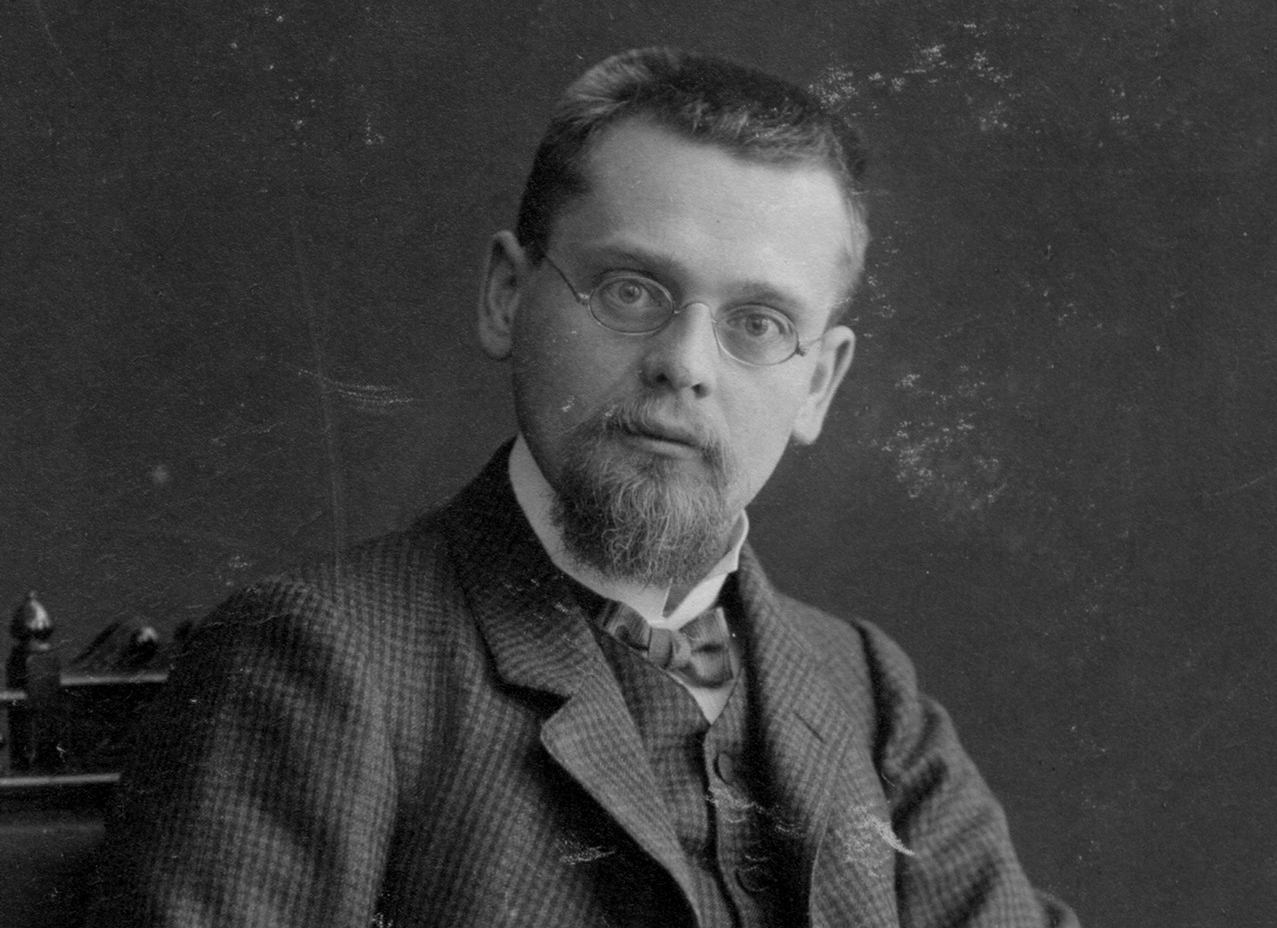
\includegraphics[width=13.5cm]{../resources/jpg/2.2.set.operations/zermelo.jpg}
    \caption*{Ernst Zermelo.}
\end{figure}
\subsection[Outermost sets in a difference is a superset.]
    {
        \color{section}Theorem 42 \color{black} : Outer sets of a difference is a superset.
    }
\documentclass[preview]{standalone}
\usepackage{amssymb, amsthm}
\usepackage{mathtools}
\usepackage{bm}


\newtheorem{theorem}{Theorem}
\renewcommand\qedsymbol{$\blacksquare$}


\begin{document}


\begin{theorem}[\textbf{2218c}]
    Let \bm{$\mathrm{A}$}, \bm{$\Lambda$}, and \bm{$\Delta$} be sets. 
    \bm{$
    \big \langle \mathrm{A} - \Lambda \big \rangle - \Delta 
        \subseteq 
    \big \langle \mathrm{A} - \Delta \big \rangle
    $}.
\end{theorem}
\begin{proof}
    Let \bm{$\lambda$} be an element in 
    \bm{$\big \langle \mathrm{A} - \Lambda \big \rangle - \Delta$}. 
    By the definition for set difference, that is
    \begin{equation*}
        \bigg[
            \Big \langle \lambda \in \mathrm{A} \Big \rangle
                \land
            \Big \langle \lambda \notin \Lambda \Big \rangle
        \bigg]
            \land
        \Big \langle \lambda \notin \Delta \Big \rangle
    \end{equation*}
    By the law of associativity for logical conjunction, 
    by the law of commutativity for logical conjunction,
    and by the simplification rule of inference,
    \begin{equation*}
        \Bigg\{
            \bigg[
                \Big \langle \lambda \in \mathrm{A} \Big \rangle
                    \land
                \Big \langle \lambda \notin \Lambda \Big \rangle
            \bigg]
                \land
            \Big \langle \lambda \notin \Delta \Big \rangle
        \Bigg\}
            \equiv
        \Bigg\{
            \bigg[
                \Big \langle \lambda \in \mathrm{A} \Big \rangle
                    \land
                \Big \langle \lambda \notin \Delta \Big \rangle
            \bigg]
                \land
            \Big \langle \lambda \notin \Lambda \Big \rangle
        \Bigg\}
    \end{equation*}
    \begin{equation*}
            \to
        \Big \langle \lambda \in \mathrm{A} \Big \rangle
            \land
        \Big \langle \lambda \notin \Delta \Big \rangle
    \end{equation*}
    $\therefore \text{\space} \bm{
    \big \langle \mathrm{A} - \Lambda \big \rangle - \Delta 
        \subseteq 
    \big \langle \mathrm{A} - \Delta \big \rangle
    }$,
    by the definitions for set difference and subsets.
\end{proof}


\end{document}
\pagebreak


% ============================= 0043 Theorem 2218d ===============================
\subsection[Alpha minus delta intersect delta $\dots$]
    {
        \color{section}Theorem 43 \color{black} : alpha minus delta intersect delta $\dots$
    }
\documentclass[preview]{standalone}
\usepackage{amssymb, amsthm}
\usepackage{mathtools}
\usepackage{bm}


\newtheorem{theorem}{Theorem}
\renewcommand\qedsymbol{$\blacksquare$}


\begin{document}


\begin{theorem}[\textbf{2218d}]
    Let \bm{$\mathrm{A}$}, \bm{$\Lambda$}, and \bm{$\Delta$} be sets. 
    \bm{$
    \big \langle \mathrm{A} - \Delta \big \rangle
        \cap 
    \big \langle \Delta - \Lambda \big \rangle
        = 
    \varnothing
    $}.
\end{theorem}
\begin{proof}
    Let \bm{$\lambda$} be an element in 
    \bm{$
    \big \langle \mathrm{A} - \Delta \big \rangle
        \cap 
    \big \langle \Delta - \Lambda \big \rangle
    $}.
    By the definitions for set difference, and set intersection, that is
    \begin{equation*}
        \bigg[
            \Big \langle \lambda \in \mathrm{A} \Big \rangle
                \land
            \Big \langle \lambda \notin \Delta \Big \rangle
        \bigg]
            \land
        \bigg[
            \Big \langle \lambda \in \Delta \Big \rangle
                \land
            \Big \langle \lambda \notin \Lambda \Big \rangle
        \bigg]
    \end{equation*}
    Since logical conjunction is associative, 
    \bm{$\lambda$} is in \bm{$\Delta$},
    and \bm{$\lambda$} is not in \bm{$\Delta$}. 
    Thus, by the negation law of logic,
    \begin{equation*}
        \Big \langle \lambda \in \mathrm{A} \Big \rangle
            \land
        \Big \langle \bot \Big \rangle
            \land
        \Big \langle \lambda \notin \Lambda \Big \rangle
    \end{equation*}
    This statement is \bm{$\bot$}, 
    by the domination law for logical conjunction. 
    And the logical identity for \bm{$\lambda \in \varnothing$} is trivially \bm{$\bot$},
    since the empty set contains no members. 
    Hence,
    \begin{equation*}
        \bigg[
            \Big \langle \lambda \in \mathrm{A} \Big \rangle
                \land
            \Big \langle \lambda \notin \Delta \Big \rangle
        \bigg]
            \land
        \bigg[
            \Big \langle \lambda \in \Delta \Big \rangle
                \land
            \Big \langle \lambda \notin \Lambda \Big \rangle
        \bigg]
            \equiv
        \Big \langle \lambda \in \varnothing \Big \rangle
    \end{equation*}
    $\therefore \text{\space} \bm{
    \big \langle \mathrm{A} - \Delta \big \rangle
        \cap 
    \big \langle \Delta - \Lambda \big \rangle
        = 
    \varnothing
    }$,
    by the definitions for the difference of sets, 
    and for the intersection of sets.
\end{proof}


\end{document}
\vspace{2\baselineskip}
\begin{figure}[!h]
    \centering
    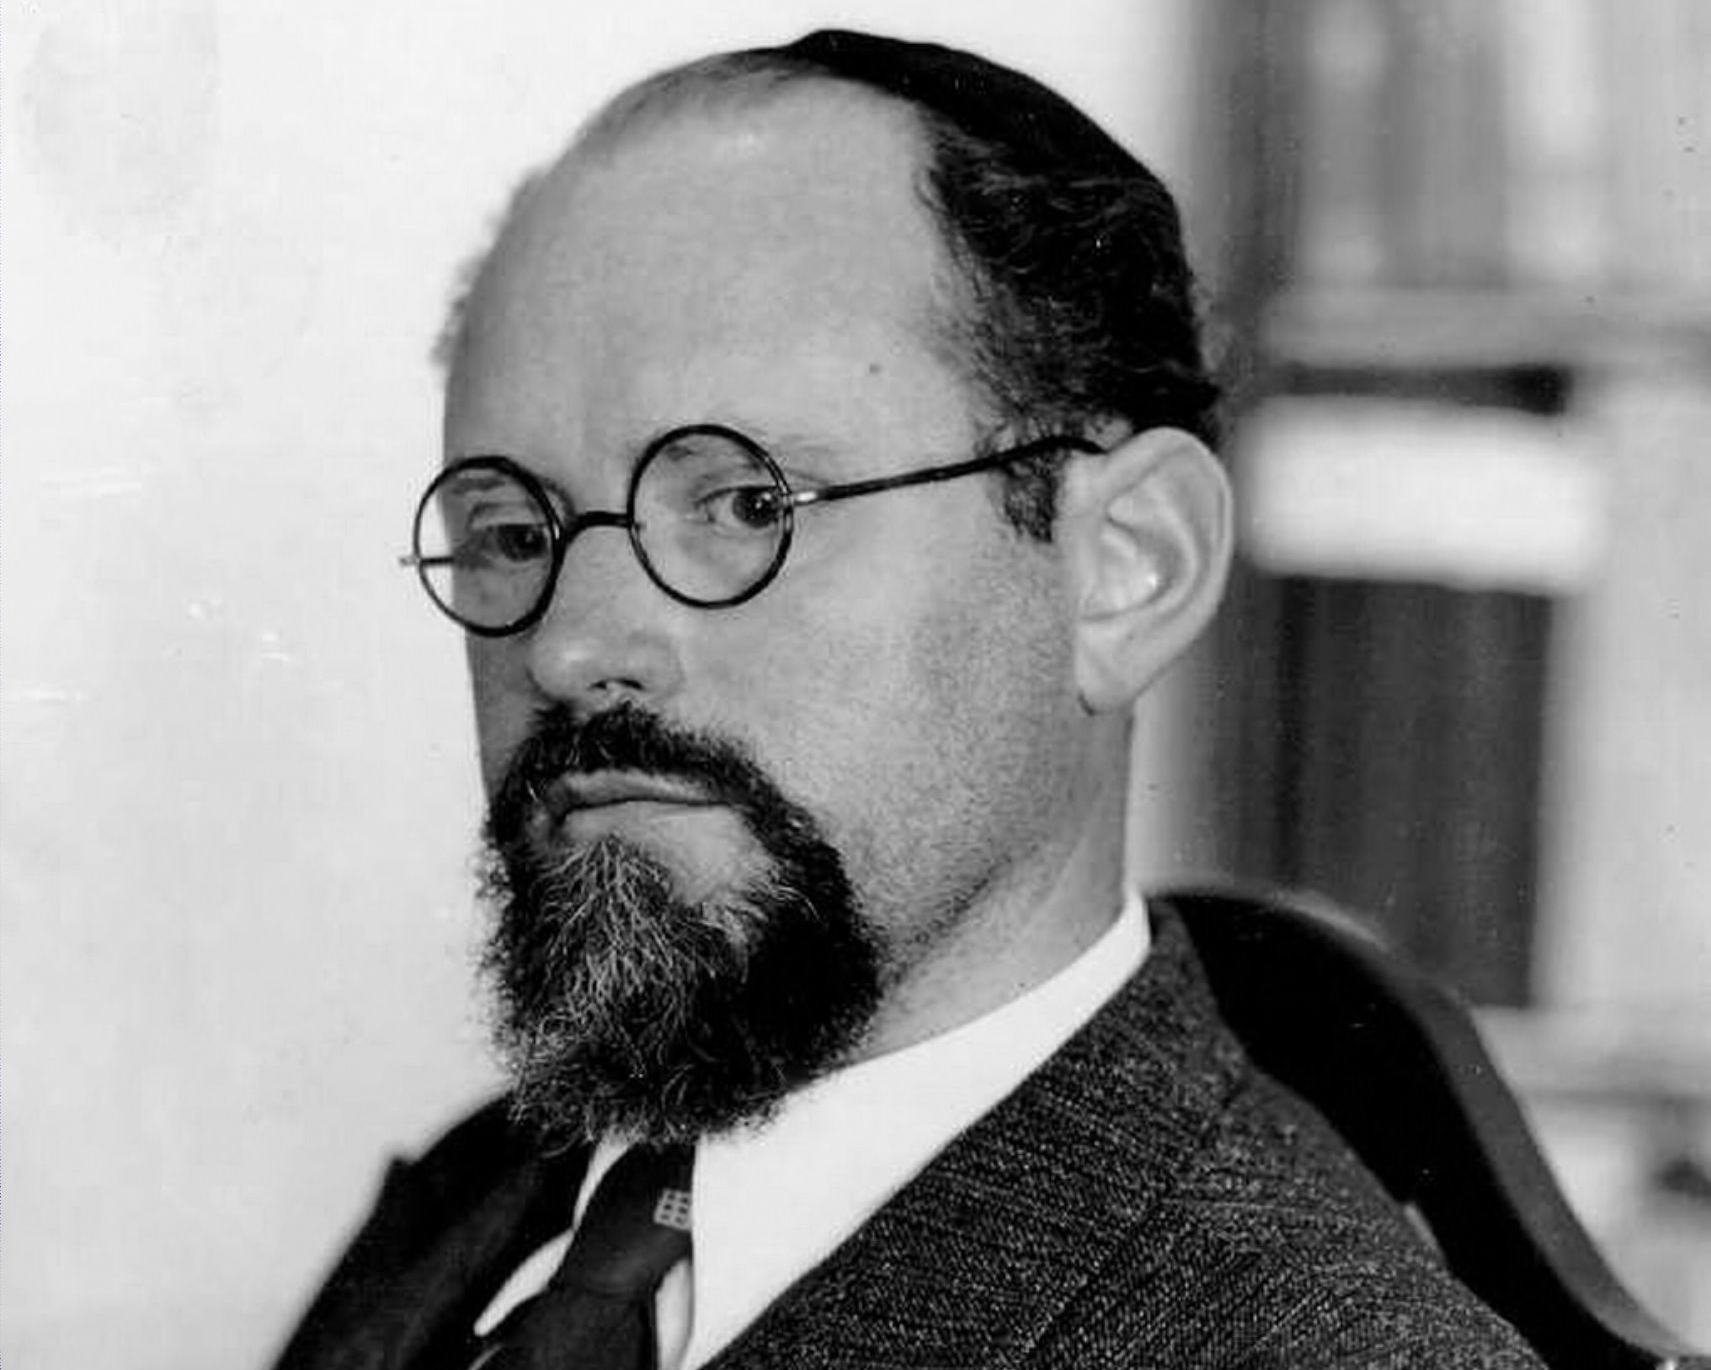
\includegraphics[width=9.5cm]{../resources/jpg/2.2.set.operations/fraenkel.jpg}
    \caption*{Abraham Fraenkel.}
\end{figure}
\pagebreak


% ============================= 0044 Theorem 2218e ===============================
\subsection[Lambda minus alpha union delta $\dots$]
    {
        \color{section}Theorem 44 \color{black} : lambda minus alpha union delta $\dots$
    }
\documentclass[preview]{standalone}
\usepackage{amssymb, amsthm}
\usepackage{mathtools}
\usepackage{bm}


\newtheorem{theorem}{Theorem}
\renewcommand\qedsymbol{$\blacksquare$}


\begin{document}


\begin{theorem}[\textbf{2218e}]
    Let \bm{$\mathrm{A}$}, \bm{$\Lambda$}, and \bm{$\Delta$} be sets. 
    \bm{$
    \big \langle \Lambda - \mathrm{A} \big \rangle 
        \cup 
    \big \langle \Delta - \mathrm{A} \big \rangle 
        = 
    \big \langle \Lambda \cup \Delta \big \rangle - \mathrm{A}
    $}.
\end{theorem}
\begin{proof} \color{black}
    Let \bm{$\lambda$} be an element in 
    \bm{$
    \big \langle \Lambda - \mathrm{A} \big \rangle 
        \cup 
    \big \langle \Delta - \mathrm{A} \big \rangle
    $}.
    By the definitions for set difference, and the union of sets, that is
    \begin{equation*}
        \bigg[
            \Big \langle \lambda \in \Lambda \Big \rangle
                \land
            \Big \langle \lambda \notin \mathrm{A} \Big \rangle
        \bigg]
            \lor
        \bigg[
            \Big \langle \lambda \in \Delta \Big \rangle
                \land
            \Big \langle \lambda \notin \mathrm{A} \Big \rangle
        \bigg]
    \end{equation*}
    Factoring \bm{$\lambda \notin \mathrm{A}$} out, 
    by the distributive laws for logical conjunction over disjunction,
    \begin{equation*}
        \Bigg\{
            \bigg[
                \Big \langle \lambda \in \Lambda \Big \rangle
                    \land
                \Big \langle \lambda \notin \mathrm{A} \Big \rangle
            \bigg]
                \lor
            \bigg[
                \Big \langle \lambda \in \Delta \Big \rangle
                    \land
                \Big \langle \lambda \notin \mathrm{A} \Big \rangle
            \bigg]
        \Bigg\}
            \equiv
    \end{equation*}
    \begin{equation*}
        \Bigg\{
            \bigg[
                \Big \langle \lambda \in \Lambda \Big \rangle
                    \lor
                \Big \langle \lambda \in \Delta \Big \rangle
            \bigg]
                \land
            \Big \langle \lambda \notin \mathrm{A} \Big \rangle
        \Bigg\}
    \end{equation*}
    $\therefore \text{\space} \bm{
    \big \langle \Lambda - \mathrm{A} \big \rangle 
        \cup 
    \big \langle \Delta - \mathrm{A} \big \rangle 
        = 
    \big \langle \Lambda \cup \Delta \big \rangle - \mathrm{A}
    }$,
    by the defintions for set difference, and set union.
\end{proof}


\end{document}
\sep
\vspace{0.5\baselineskip}


% ============================= 0045 Theorem 2219 ================================
\subsection[Alpha intersect complement lambda.]
    {
        \color{section}Theorem 45 \color{black} : alpha intersect complement lambda.
    }
\documentclass[preview]{standalone}
\usepackage{amssymb, amsthm}
\usepackage{mathtools}
\usepackage{bm}


\newtheorem{theorem}{Theorem}
\renewcommand\qedsymbol{$\blacksquare$}


\begin{document}


\begin{theorem}[\textbf{2219}]
    Let \bm{$\mathrm{A}$}, and \bm{$\Lambda$} be sets. 
    \bm{$
    \mathrm{A} - \Lambda 
        = 
    \mathrm{A} \cap \overline{\Lambda}
    $}.
\end{theorem}
\begin{proof}
    Let \bm{$\lambda$} be an element in \bm{$\mathrm{A} - \Lambda$}. 
    By the definition for set difference,
    \begin{equation*}
        \Big \langle \lambda \in \mathrm{A} \Big \rangle
            \land
        \Big \langle \lambda \notin \Lambda \Big \rangle
    \end{equation*}
    By the definition for set complementation,
    \begin{equation*}
        \bigg[
            \Big \langle \lambda \in \mathrm{A} \Big \rangle
                \land
            \Big \langle \lambda \notin \Lambda \Big \rangle
        \bigg]
            \equiv
        \bigg[
            \Big \langle \lambda \in \mathrm{A} \Big \rangle
                \land
            \Big \langle \lambda \in \overline{\Lambda} \Big \rangle
        \bigg]
    \end{equation*}
    $\therefore \text{\space} \bm{
    \mathrm{A} - \Lambda 
        = 
    \mathrm{A} \cap \overline{\Lambda}
    }$,
    by the definition for the intersection of sets.
\end{proof}


\end{document}
\pagebreak


% ============================= 0046 Theorem 2220 ================================
\subsection[An identity for the set alpha.]
    {
        \color{section}Theorem 46 \color{black} : an identity for the set alpha.
    }
\documentclass[preview]{standalone}
\usepackage{amssymb, amsthm}
\usepackage{mathtools}
\usepackage{bm}


\newtheorem{theorem}{Theorem}
\renewcommand\qedsymbol{$\blacksquare$}


\begin{document}


\begin{theorem}[\textbf{2220}]
    Let \bm{$\mathrm{A}$}, and \bm{$\Lambda$} be sets. 
    \bm{$
    \big \langle \mathrm{A} \cap \Lambda \big \rangle 
        \cup 
    \big \langle \mathrm{A} \cap \overline{\Lambda} \big \rangle 
        = 
    \mathrm{A}
    $}.
\end{theorem}
\begin{proof}
    Let \bm{$\lambda$} be an element in 
    \bm{$
    \big \langle \mathrm{A} \cap \Lambda \big \rangle 
        \cup 
    \big \langle \mathrm{A} \cap \overline{\Lambda} \big \rangle
    $}.
    By the definitions for the union of sets, and set intersection, that is,
    \begin{equation*}
        \bigg[
            \Big \langle \lambda \in \mathrm{A} \Big \rangle
                \land
            \Big \langle \lambda \in \Lambda \Big \rangle
        \bigg]
            \lor
        \bigg[
            \Big \langle \lambda \in \mathrm{A} \Big \rangle
                \land
            \Big \langle \lambda \in \overline{\Lambda} \Big \rangle
        \bigg]
    \end{equation*} 
    By the law of distribution for logical conjunction over disjunction,
    we can factor out the term \bm{$\lambda \in \mathrm{A}$}. 
    Hence, the following statement is equivalent,
    \begin{equation*}
        \Big \langle \lambda \in \mathrm{A} \Big \rangle
            \land
        \bigg[
            \Big \langle \lambda \in \Lambda \Big \rangle
                \lor
            \Big \langle \lambda \in \overline{\Lambda} \Big \rangle
        \bigg]
    \end{equation*}
    \bm{$
    \lambda \in \Lambda 
        \lor 
    \lambda \in \overline{\Lambda} 
        \equiv 
    \top
    $},
    by the negation laws of logic.
    Thus, by the identity law for logical conjunction,
    \begin{equation*}
        \Bigg\{
            \bigg[
                \Big \langle \lambda \in \mathrm{A} \Big \rangle
                    \land
                \Big \langle \lambda \in \Lambda \Big \rangle
            \bigg]
                \lor
            \bigg[
                \Big \langle \lambda \in \mathrm{A} \Big \rangle
                    \land
                \Big \langle \lambda \in \overline{\Lambda} \Big \rangle
            \bigg]
        \Bigg\}
            \equiv
        \Bigg\{
            \Big \langle \lambda \in \mathrm{A} \Big \rangle
                \land
            \Big \langle \top \Big \rangle
        \Bigg\}
            \equiv
    \end{equation*}
    \begin{equation*}
        \Big \langle \lambda \in \mathrm{A} \Big \rangle
    \end{equation*}
    $
    \therefore \text{\space} \bm{
    \big \langle \mathrm{A} \cap \Lambda \big \rangle 
        \cup 
    \big \langle \mathrm{A} \cap \overline{\Lambda} \big \rangle
        = 
    \mathrm{A}
    }$.
\end{proof}


\end{document}
\sep


% ============================= 0047 Theorem 2221 ================================
\subsection[The associative law for set union.]
    {
        \color{section}Theorem 47 \color{black} : the associative law for set union.
    }
\documentclass[preview]{standalone}
\usepackage{amssymb, amsthm}
\usepackage{mathtools}
\usepackage{bm}


\newtheorem{theorem}{Theorem}
\renewcommand\qedsymbol{$\blacksquare$}


\begin{document}


\begin{theorem}[\textbf{2221}]
    Let \bm{$\mathrm{A}$}, \bm{$\Lambda$}, and \bm{$\Delta$} be sets. 
    Set union is associative such that
    \begin{equation*}
        \bm{
            \mathrm{A} 
                \cup 
            \big \langle \Lambda \cup \Delta \big \rangle 
                = 
            \big \langle \mathrm{A} \cup \Lambda \big \rangle 
                \cup 
            \Delta
        } 
    \end{equation*}
\end{theorem}
\begin{proof}
    Let \bm{$\lambda$} be an element in 
    \bm{$
    \mathrm{A} 
        \cup 
    \big \langle \Lambda \cup \Delta \big \rangle
    $}. 
    By the definition for the union of sets, that is
    \begin{equation*}
        \Big \langle \lambda \in \mathrm{A} \Big \rangle
            \lor
        \bigg[
            \Big \langle \lambda \in \Lambda \Big \rangle
                \lor
            \Big \langle \lambda \in \Delta \Big \rangle
        \bigg]
    \end{equation*}
    It trivially follows from the associative law for logical disjunction that
    \begin{equation*}
        \Big \langle \lambda \in \mathrm{A} \Big \rangle
            \lor
        \bigg[
            \Big \langle \lambda \in \Lambda \Big \rangle
                \lor
            \Big \langle \lambda \in \Delta \Big \rangle
        \bigg]
            \equiv
        \bigg[
            \Big \langle \lambda \in \mathrm{A} \Big \rangle
                \lor
            \Big \langle \lambda \in \Lambda \Big \rangle
        \bigg]
            \lor
        \Big \langle \lambda \in \Delta \Big \rangle
    \end{equation*}
    $\therefore \text{\space} \bm{
    \mathrm{A} 
        \cup 
    \big \langle \Lambda \cup \Delta \big \rangle 
        = 
    \big \langle \mathrm{A} \cup \Lambda \big \rangle 
        \cup 
    \Delta
    }$, 
    such that set union is associative.
    by the definition for the union of sets.
\end{proof}


\end{document}
\pagebreak


% ============================= 0048 Theorem 2222 ================================
\subsection[The associative law for set intersection.]
    {
        \color{section}Theorem 48 \color{black} : the associative law for set intersection.
    }
\documentclass[preview]{standalone}
\usepackage{amssymb, amsthm}
\usepackage{mathtools}
\usepackage{bm}


\newtheorem{theorem}{Theorem}
\renewcommand\qedsymbol{$\blacksquare$}


\begin{document}


\begin{theorem}[\textbf{2222}]
    Let \bm{$\mathrm{A}$}, \bm{$\Lambda$}, and \bm{$\Delta$} be sets. 
    Set intersection is associative such that
    \begin{equation*}
        \bm{
            \mathrm{A} 
                \cap 
            \big \langle \Lambda \cap \Delta \big \rangle 
                = 
            \big \langle \mathrm{A} \cap \Lambda \big \rangle
                \cap 
            \Delta
        }
\end{equation*}
\end{theorem}
\begin{proof}
    Let \bm{$\lambda$} be an element in 
    \bm{$
    \mathrm{A} 
        \cap 
    \big \langle \Lambda \cap \Delta \big \rangle
    $}. 
    By the definition for the intersection of sets, that is 
    \begin{equation*}
        \Big \langle \lambda \in \mathrm{A} \Big \rangle
            \land
        \bigg[
            \Big \langle \lambda \in \Lambda \Big \rangle
                \land
            \Big \langle \lambda \in \Delta \Big \rangle
        \bigg]
    \end{equation*}
    It trivially follows from the associative law for logical conjunction that
    \begin{equation*}
        \Big \langle \lambda \in \mathrm{A} \Big \rangle
            \land
        \bigg[
            \Big \langle \lambda \in \Lambda \Big \rangle
                \land
            \Big \langle \lambda \in \Delta \Big \rangle
        \bigg]
            \equiv
        \bigg[
            \Big \langle \lambda \in \mathrm{A} \Big \rangle
                \land
            \Big \langle \lambda \in \Lambda \Big \rangle
        \bigg]
            \land
        \Big \langle \lambda \in \Delta \Big \rangle
    \end{equation*}
    $
    \therefore \text{\space} \bm{
    \mathrm{A} 
        \cap 
    \big \langle \Lambda \cap \Delta \big \rangle 
        = 
    \big \langle \mathrm{A} \cap \Lambda \big \rangle
        \cap 
    \Delta
    }$,
    such that set intersection is associative,
    by the definition for the intersection of sets.
\end{proof}


\end{document}
\vspace{2.5\baselineskip}
\begin{figure}[!h]
    \centering
    
\includegraphics[width=7cm]{../resources/jpg/2.2.set.operations/border7.jpg}
\end{figure}
\vspace{2\baselineskip}


% ============================= 0049 Theorem 2223 ================================
\subsection[Union is distributive over intersection.]
    {
        \color{section}Theorem 49 \color{black} : union is distributive over intersection.
    }
\documentclass[preview]{standalone}
\usepackage{amssymb, amsthm}
\usepackage{mathtools}
\usepackage{bm}


\newtheorem{theorem}{Theorem}
\renewcommand\qedsymbol{$\blacksquare$}


\begin{document}


\begin{theorem}[\textbf{2223}]
    Let \bm{$\mathrm{A}$}, \bm{$\Lambda$}, and \bm{$\Delta$} be sets.
    Set union is distributive over set intersection such that
    \begin{equation*}
        \bm{
            \mathrm{A} \cup \Big \langle \Lambda \cap \Delta \Big \rangle 
                =
            \Big \langle \mathrm{A} \cup \Lambda \Big \rangle
                \cap 
            \Big \langle \mathrm{A} \cup \Delta \Big \rangle
        }
    \end{equation*}
\end{theorem}
\begin{proof}
    Let \bm{$\lambda$} be an element in 
    \bm{$
    \mathrm{A} \cup \big \langle \Lambda \cap \Delta \big \rangle
    $}.
    By the defintions for the union and intersection of sets, that is 
    \begin{equation*}
        \big \langle \lambda \in \mathrm{A} \big \rangle
            \lor
        \Big[
            \big \langle \lambda \in \Lambda \big \rangle
                \land
            \big \langle \lambda \in \Delta \big \rangle
        \Big]
    \end{equation*}
    By the law of distribution for logical disjunction over conjunction,
    \begin{equation*}
        \big \langle \lambda \in \mathrm{A} \big \rangle
            \lor
        \Big[
            \big \langle \lambda \in \Lambda \big \rangle
                \land
            \big \langle \lambda \in \Delta \big \rangle
        \Big] 
            \equiv
        \Big[
            \big \langle \lambda \in \mathrm{A} \big \rangle
                \lor
            \big \langle \lambda \in \Lambda \big \rangle
        \Big]
            \land
        \Big[
            \big \langle \lambda \in \mathrm{A} \big \rangle
                \lor
            \big \langle \lambda \in \Delta \big \rangle
        \Big]
    \end{equation*}
    $\therefore \text{\space} \bm{
    \mathrm{A} \cup \big \langle \Lambda \cap \Delta \big \rangle 
        = 
    \big \langle \mathrm{A} \cup \Lambda \big \rangle
        \cap 
    \big \langle \mathrm{A} \cup \Delta \big \rangle
    }$, 
    such that set union is distributive over set intersection,
    by the definitons for set union and set intersection.
\end{proof}


\end{document}
\pagebreak


% ============================= 0050 Theorem 2224 ================================
\subsection[The distribution of differences.]
    {
        \color{section}Theorem 50 \color{black} : the distribution of differences.
    }
\documentclass[preview]{standalone}
\usepackage{amssymb, amsthm}
\usepackage{mathtools}
\usepackage{bm}


\newtheorem{theorem}{Theorem}
\renewcommand\qedsymbol{$\blacksquare$}


\begin{document}


\begin{theorem}[\textbf{2224}]
    Let \bm{$\mathrm{A}$}, \bm{$\Lambda$}, and \bm{$\Delta$} be sets. 
    \begin{equation*}
        \bm{
            \Big \langle \mathrm{A} - \Lambda \Big \rangle - \Delta 
                = 
            \Big \langle \mathrm{A} - \Delta \Big \rangle 
                - 
            \Big \langle \Lambda - \Delta \Big \rangle
        }
    \end{equation*}
\end{theorem}
\begin{proof}
    Let \bm{$\lambda$} be an element in 
    \bm{$
    \big \langle \mathrm{A} - \Lambda \big \rangle - \Delta 
    $}. 
    By the definition for set difference,
    \begin{equation*}
        \bigg[
            \Big \langle \lambda \in \mathrm{A} \Big \rangle
                \land
            \Big \langle \lambda \notin \Lambda \Big \rangle
        \bigg]
            \land
        \Big \langle \lambda \notin \Delta \Big \rangle
    \end{equation*}
    Note that, by the indentity law for logical disjunction, 
    \bm{$
    \lambda \notin \Lambda
        \equiv 
    \lambda \notin \Lambda
        \lor 
    \bot
    $}.
    And since
    \bm{$
    \lambda \in \Delta
        \equiv 
    \bot
    $},
    by definition,
    it follows that
    \begin{equation*}
        \Big \langle \lambda \notin \Lambda \Big \rangle
            \equiv
        \bigg[
            \Big \langle \lambda \notin \Lambda \Big \rangle
                \lor
            \Big \langle \bot \Big \rangle
        \bigg]
            \equiv
        \bigg[
            \Big \langle \lambda \notin \Lambda \Big \rangle
                \lor
            \Big \langle \lambda \in \Delta \Big \rangle
        \bigg]
    \end{equation*}
    Moreover, by the double negation law of logic, and by DeMorgans laws,
    \begin{equation*}
        \Big \langle \lambda \notin \Lambda \Big \rangle
            \equiv
        \lnot \Bigg\{
            \lnot \bigg[
                \Big \langle \lambda \notin \Lambda \Big \rangle
                    \lor
                \Big \langle \lambda \in \Delta \Big \rangle
            \bigg]
        \Bigg\}
            \equiv
        \lnot \bigg[
            \Big \langle \lambda \in \Lambda \Big \rangle
                \land
            \Big \langle \lambda \notin \Delta \Big \rangle
        \bigg]
    \end{equation*}
    Thus, the proposition
    \bm{$
    \lambda \in
    \big \langle \mathrm{A} - \Lambda \big \rangle - \Delta 
    $},
    is equivalent to
    \begin{equation*}
        \Bigg\{
        \Big \langle \lambda \in \mathrm{A} \Big \rangle
            \land
        \lnot \bigg[
            \Big \langle \lambda \in \Lambda \Big \rangle
                \land
            \Big \langle \lambda \notin \Delta \Big \rangle
        \bigg]
        \Bigg\}
            \land
        \Big \langle \lambda \notin \Delta \Big \rangle
    \end{equation*}
    By law of commutativity (and association) for logical conjunction, 
    that is
    \begin{equation*}
        \bigg[
            \Big \langle \lambda \in \mathrm{A} \Big \rangle
                \land
            \Big \langle \lambda \notin \Delta \Big \rangle
        \bigg]
            \land
        \lnot \bigg[
            \Big \langle \lambda \in \Lambda \Big \rangle
                \land
            \Big \langle \lambda \notin \Delta \Big \rangle
        \bigg]
    \end{equation*}
    By the definitions for the difference of sets, set complementation,
    and the intersection of sets,
    \begin{equation*}
        \bigg[
        \Big \langle \mathrm{A} - \Lambda \Big \rangle - \Delta
        \bigg]
            \equiv
        \bigg[
        \Big \langle \mathrm{A} - \Delta \Big \rangle
            \cap
        \overline{
            \Big \langle \Lambda - \Delta \Big \rangle
        }
        \bigg]
    \end{equation*}
    $\therefore \text{\space} \bm{
    \big \langle \mathrm{A} - \Lambda \big \rangle - \Delta 
        = 
    \big \langle \mathrm{A} - \Delta \big \rangle 
        - 
    \big \langle \Lambda - \Delta \big \rangle
    }$, by Thereom 45.

\end{proof}


\end{document}
\sep
\pagebreak


% ============================= 0051 Theorem 2231 ================================
\subsection[Subsets are contrapositive.]
    {
        \color{section}Theorem 51 \color{black} : Subsets are contrapositive.
    }
\documentclass[preview]{standalone}
\usepackage{amssymb, amsthm}
\usepackage{mathtools}
\usepackage{bm}


\newtheorem{theorem}{Theorem}
\renewcommand\qedsymbol{$\blacksquare$}


\begin{document}


\begin{theorem}[\textbf{2231}]
    Let \bm{$\mathrm{A}$}, and \bm{$\Lambda$} be subsets of a universal set \bm{$\Omega$}. 
    \begin{equation*}
        \bm{
            \mathrm{A} \subseteq \Lambda
                \text{ if and only if } 
            \overline{\Lambda} \subseteq \overline{\mathrm{A}}
            }
    \end{equation*}
\end{theorem}
\begin{proof}
    The proposition \bm{$\mathrm{A} \subseteq \Lambda$} is defined by the universal quantification% statement 
    \begin{equation*}
        \forall \lambda \Big \langle \lambda \in \mathrm{A} \rightarrow \lambda \in \Lambda \Big \rangle
    \end{equation*}
    Where \bm{$\lambda$} is an element in the domain of discourse \bm{$\Omega$}.
    It is a tautology that the truth value for the predicate is equivalent to its contrapositive. 
    Thus,  
    \begin{equation*}
        \forall \lambda \Big \langle \lambda \notin \Lambda \rightarrow \lambda \notin \mathrm{A} \Big \rangle
    \end{equation*} 
    By the definition for set complementation, and subsets
    \bm{$\lambda \in \overline{\Lambda} \subseteq \overline{\mathrm{A}}$} 
    $\therefore$ \bm{$\mathrm{A} \subseteq \Lambda$} \textbf{\emph{ iff }} \bm{$\overline{\Lambda} \subseteq \overline{\mathrm{A}}$}.
\end{proof}


\end{document}
\vspace{2.5\baselineskip}
\begin{figure}[!h]
    \centering
    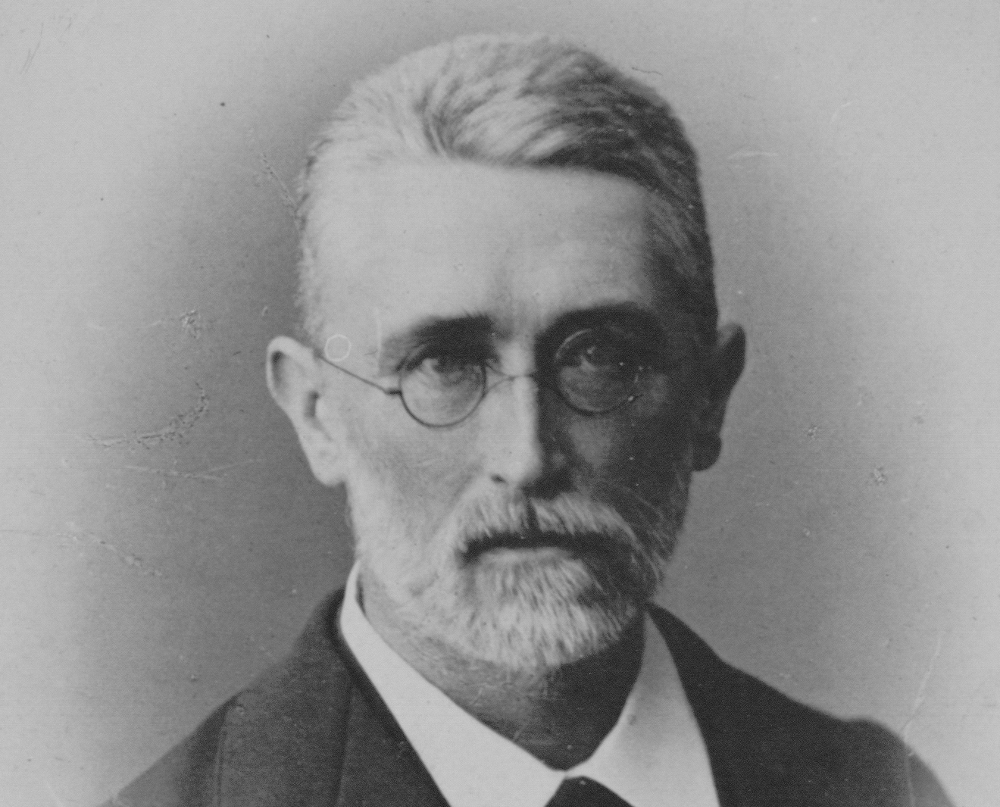
\includegraphics[width=13cm]{../resources/jpg/2.2.set.operations/dedekind.png}
    \caption*{Richard Dedekind.}
\end{figure}
\pagebreak


% ============================= 0052 Theorem 2235 ================================
\subsection[Symmetric difference is a set difference.]
    {
        \color{section}Theorem 52 \color{black} : symmetric difference is a set difference.
    }
\documentclass[preview]{standalone}
\usepackage{amssymb, amsthm}
\usepackage{mathtools}
\usepackage{bm}


\newtheorem{theorem}{Theorem}
\renewcommand\qedsymbol{$\blacksquare$}


\begin{document}


\begin{theorem}[\textbf{2235}]
    Let \bm{$\mathrm{A}$}, and \bm{$\Lambda$} be sets. 
    \bm{$
    \mathrm{A} \oplus \Lambda 
        = 
    \big \langle \mathrm{A} \cup \Lambda \big \rangle 
        - 
    \big \langle \mathrm{A} \cap \Lambda \big \rangle
    $}.
\end{theorem}
\begin{proof}
    Let \bm{$\lambda$} be an element in \bm{$\mathrm{A} \oplus \Lambda$}. 
    By the definition for the symmetric difference of sets,
    \begin{equation*}
        \bigg[
            \Big \langle \lambda \in \mathrm{A} \Big \rangle 
                \land 
            \Big \langle \lambda \notin \Lambda \Big \rangle
        \bigg] 
            \lor 
        \bigg[
            \Big \langle \lambda \notin \mathrm{A} \Big \rangle
                \land 
            \Big \langle \lambda \in \Lambda \Big \rangle
        \bigg]
    \end{equation*}
    Distributing the right-hand side over the left-hand side,
    by the distributive laws of logic, that is
    \begin{equation*}
        \Bigg\{
            \Big \langle \lambda \in \mathrm{A} \Big \rangle
                \lor
            \bigg[
                \Big \langle \lambda \notin \mathrm{A} \Big \rangle
                    \land 
                \Big \langle \lambda \in \Lambda \Big \rangle
            \bigg]
        \Bigg\}
            \land
        \Bigg\{
            \Big \langle \lambda \notin \Lambda \Big \rangle
                \lor
            \bigg[
                \Big \langle \lambda \notin \mathrm{A} \Big \rangle
                    \land 
                \Big \langle \lambda \in \Lambda \Big \rangle
            \bigg]
        \Bigg\}
    \end{equation*}
    Again, by the distributive law for logical disjunction over conjunction,
    and by the associative law for logical conjunction, we have
    \begin{equation*}
        \bigg[
            \Big \langle \lambda \in \mathrm{A} \Big \rangle
                \lor
            \Big \langle \lambda \notin \mathrm{A} \Big \rangle
        \bigg]
            \land
        \bigg[
            \Big \langle \lambda \in \mathrm{A} \Big \rangle
                \lor 
            \Big \langle \lambda \in \Lambda \Big \rangle
        \bigg]
            \land
        \bigg[
            \Big \langle \lambda \notin \Lambda \Big \rangle
                \lor
            \Big \langle \lambda \notin \mathrm{A} \Big \rangle
        \bigg]
            \land
    \end{equation*}
    \begin{equation*}
        \bigg[
            \Big \langle \lambda \notin \Lambda \Big \rangle
                \lor 
            \Big \langle \lambda \in \Lambda \Big \rangle
        \bigg]
    \end{equation*}
    The following identity is given by the negation laws of logic,
    \begin{equation*}
        \big \langle \top \big \rangle
            \land
        \bigg[
            \Big \langle \lambda \in \mathrm{A} \Big \rangle
                \lor 
            \Big \langle \lambda \in \Lambda \Big \rangle
        \bigg]
            \land
        \bigg[
            \Big \langle \lambda \notin \Lambda \Big \rangle
                \lor
            \Big \langle \lambda \notin \mathrm{A} \Big \rangle
        \bigg]
            \land
        \big \langle \top \big \rangle
    \end{equation*}
    By DeMorgans laws,
    and by the identity law for logical conjunction, 
    that is
    \begin{equation*}
        \bigg[
            \Big \langle \lambda \in \mathrm{A} \Big \rangle
                \lor 
            \Big \langle \lambda \in \Lambda \Big \rangle
        \bigg]
            \land
        \lnot \bigg[
            \Big \langle \lambda \in \Lambda \Big \rangle
                \land
            \Big \langle \lambda \in \mathrm{A} \Big \rangle
        \bigg]
    \end{equation*}
    Which, by the definitions for set union, set intersection,
    and set membership, is equivalent to
    \begin{equation*}
        \Bigg\{
            \lambda \in \Big \langle \mathrm{A} \cup \Lambda \Big \rangle
                \land
            \lnot \bigg[ 
                \lambda \in \Big \langle \Lambda \cap \mathrm{A} \Big \rangle
            \bigg]
        \Bigg\}
            \equiv
        \Bigg\{
            \lambda \in \Big \langle \mathrm{A} \cup \Lambda \Big \rangle
                \land
            \lambda \notin \Big \langle \Lambda \cap \mathrm{A} \Big \rangle
        \Bigg\}
    \end{equation*}
    $\therefore$ by the definition for set difference,
    \bm{$
    \mathrm{A} \oplus \Lambda 
        = 
    \big \langle \mathrm{A} \cup \Lambda \big \rangle 
        - 
    \big \langle \mathrm{A} \cap \Lambda \big \rangle
    $}.
\end{proof}


\end{document}
\sep
\pagebreak


% ============================= 0053 Theorem 2236 ================================
\subsection[Symmetric difference is a union.]
    {
        \color{section}Theorem 53 \color{black} : symmetric difference is a union.
    }
\documentclass[preview]{standalone}
\usepackage{amssymb, amsthm}
\usepackage{mathtools}
\usepackage{bm}


\newtheorem{theorem}{Theorem}
\renewcommand\qedsymbol{$\blacksquare$}


\begin{document}


\begin{theorem}[\textbf{2236}]
    Let \bm{$\Gamma$}, and \bm{$\Xi$} be sets. 
    \begin{equation*}
        \bm{
            \Gamma \oplus \Xi 
                = 
            \Big \langle \Gamma - \Xi \Big \rangle
                \cup 
            \Big \langle \Xi - \Gamma \Big \rangle
        }
    \end{equation*}
\end{theorem}
\begin{proof}
    Suppose there exists an element \bm{$\zeta$} such that \bm{$\zeta$} is a member of \bm{$\Gamma \oplus \Xi$}. 
    By the definition for symmetric difference,
    \begin{equation*}
        \bigg[
            \Big \langle \zeta \in \Gamma \Big \rangle 
                \land 
            \Big \langle \zeta \notin \Xi \Big \rangle
        \bigg] 
            \lor 
        \bigg[
            \Big \langle \zeta \notin \Gamma \Big \rangle
                \land 
            \Big \langle \zeta \in \Xi \Big \rangle
        \bigg]   
    \end{equation*}
    Because logical conjunction is associative, this statement is equivalent to 
    \begin{equation*}
        \bigg[
            \Big \langle \zeta \in \Gamma \Big \rangle 
                \land 
            \Big \langle \zeta \notin \Xi \Big \rangle
        \bigg] 
            \lor 
        \bigg[
            \Big \langle \zeta \in \Xi \Big \rangle
                \land 
            \Big \langle \zeta \notin \Gamma \Big \rangle
        \bigg]   
    \end{equation*}
    $\therefore \text{\space} \bm{
        \Gamma \oplus \Xi 
        = 
    \big \langle \Gamma - \Xi \big \rangle
        \cup 
    \big \langle \Xi - \Gamma \big \rangle
    }$, by the defintions for set union and the difference of sets.
\end{proof}


\end{document}
\sep


% ============================= 0054 Theorem 2237a ===============================
\subsection[Symmetric difference between a set and itself.]
    {
        \color{section}Theorem 54 \color{black} : symmetric difference of a set itself.
    }
\documentclass[preview]{standalone}
\usepackage{amssymb, amsthm}
\usepackage{mathtools}
\usepackage{bm}


\newtheorem{theorem}{Theorem}
\renewcommand\qedsymbol{$\blacksquare$}


\begin{document}


\begin{theorem}[\textbf{2237a}]
    Let \bm{$\Gamma$} be a subset of the universal set \bm{$\Omega$}. 
    \begin{equation*}
        \bm{\Gamma \oplus \Gamma = \varnothing}
    \end{equation*}
\end{theorem}
\begin{proof}
    By Theorem 52, 
    \bm{$
    \Gamma \oplus \Gamma 
        = 
    \big \langle \Gamma \cup \Gamma \big \rangle
        - 
    \big \langle \Gamma \cap \Gamma \big \rangle
    $}. 
    By the set idempotent laws, 
    that is \bm{$\Gamma - \Gamma$}, 
    and by Theorem 45, equivalent to 
    \bm{$\Gamma \cap \overline{\Gamma}$}. 
    It follows immediately from the set complement law for the intersection of sets that 
    \bm{$\Gamma \oplus \Gamma = \varnothing$}.
\end{proof}


\end{document}
\sep


% ============================= 0055 Theorem 2237b ===============================
\subsection[Symmetric difference with the empty set.]
    {
        \color{section}Theorem 55 \color{black} : symmetric difference with the empty set.
    }
\documentclass[preview]{standalone}
\usepackage{amssymb, amsthm}
\usepackage{mathtools}
\usepackage{bm}


\newtheorem{theorem}{Theorem}
\renewcommand\qedsymbol{$\blacksquare$}


\begin{document}


\begin{theorem}[\textbf{2237b}]
    Let \bm{$\Gamma$} be a subset of the universal set \bm{$\Omega$}. 
    \begin{equation*}
        \bm{\Gamma \oplus \varnothing = \Gamma}
    \end{equation*}
\end{theorem}
\begin{proof}
    By Theorem 52, 
    \bm{$
    \Gamma \oplus \varnothing 
        = 
    \big \langle \Gamma \cup \varnothing \big \rangle
        - 
    \big \langle \Gamma \cap \varnothing \big \rangle
    $}. 
    By the identity law for set union, 
    and by the set domination law for intersection, 
    that is \bm{$\Gamma - \varnothing$}, 
    which by Theorem 45 means 
    \bm{$\Gamma \cap \overline{\bm{\varnothing}}$}. 
    Because \bm{$\overline{\bm{\varnothing}} = \Omega$},
    \bm{$\Gamma \cap \overline{\bm{\varnothing}} \equiv \Gamma \cap \Omega}$. 
    Thus, by the set identity law for intersection, 
    \bm{$\Gamma \oplus \varnothing = \Gamma$}.
\end{proof}


\end{document}
\pagebreak


% ============================= 0056 Theorem 2237c ===============================
\subsection[Symmetric difference with the universe.]
    {
        \color{section}Theorem 56 \color{black} : symmetric difference with the universe.
    }
\documentclass[preview]{standalone}
\usepackage{amssymb, amsthm}
\usepackage{mathtools}
\usepackage{bm}


\newtheorem{theorem}{Theorem}
\renewcommand\qedsymbol{$\blacksquare$}


\begin{document}


\begin{theorem}[\textbf{2237c}]
    Let \bm{$\Gamma$} be a subset of the universal set \bm{$\Omega$}. 
    \begin{equation*}
        \bm{\Gamma \oplus \Omega = \overline{\Gamma}}
    \end{equation*}
\end{theorem}
\begin{proof}
    By Theorem 52, 
    \bm{$
    \Gamma \oplus \Omega
        = 
    \big \langle \Gamma \cup \Omega \big \rangle
        - 
    \big \langle \Gamma \cap \Omega \big \rangle
    $}. 
    By the set domination law for set union, and by the set 
    identity law for set intersection, that is \bm{$\Omega - \Gamma$}. 
    Hence, by Theorem 45, 
    \bm{$\Omega \cap \overline{\Gamma}$}.
    By the identity law for set intersection,
    \bm{$\Gamma \oplus \Omega = \overline{\Gamma}$}.
\end{proof}


\end{document}
\sep


% ============================= 0057 Theorem 2237d ===============================
\subsection[Symmetric difference with a complement.]
    {
        \color{section}Theorem 57 \color{black} : symmetric difference and a complement.
    }
\documentclass[preview]{standalone}
\usepackage{amssymb, amsthm}
\usepackage{mathtools}
\usepackage{bm}


\newtheorem{theorem}{Theorem}
\renewcommand\qedsymbol{$\blacksquare$}


\begin{document}


\begin{theorem}[\textbf{2237d}]
    Let \bm{$\Xi$} be a subset of a universal set \bm{$\Omega$}. 
    \begin{equation*}
        \bm{\Xi \oplus \overline{\Xi} = \Omega}
    \end{equation*}
\end{theorem}
\begin{proof}
    By Theorem 52, 
    \bm{$
    \Xi \oplus \overline{\Xi} 
        = 
    \big \langle \Xi \cup \overline{\Xi} \big \rangle
        - 
    \big \langle \Xi \cap \overline{\Xi} \big \rangle
    $}. 
    By the set complement laws that is \bm{$\Omega - \varnothing$}. 
    Rather, \bm{$\Omega \cap \overline{\bm{\varnothing}}$}, 
    by Theorem 45. 
    Since \bm{$\overline{\bm{\varnothing}} = \Omega$}, that is 
    \bm{$\Omega \cap \Omega$}. Which is \bm{$\Omega$}, 
    by the idempotent law for set intersection.
    Thus, \bm{$\Xi \oplus \overline{\Xi} = \Omega$}.
\end{proof}


\end{document}
\begin{figure}[!h]
    \centering
    
\includegraphics[width=3cm]{../resources/jpg/2.2.set.operations/horus.png}
\end{figure}


% ============================= 0058 Theorem 2238a ===============================
\subsection[Symmetric difference is associative.]
    {
        \color{section}Theorem 58 \color{black} : symmetric difference is associative.
    }
\documentclass[preview]{standalone}
\usepackage{amssymb, amsthm}
\usepackage{mathtools}
\usepackage{bm}


\newtheorem{theorem}{Theorem}
\renewcommand\qedsymbol{$\blacksquare$}


\begin{document}


\begin{theorem}[\textbf{2238a}]
    Let \bm{$\mathrm{A}$}, and \bm{$\Lambda$} be sets. 
    Symmetric difference of sets is associative such that 
    \begin{equation*}
        \bm{
            \big \langle \mathrm{A} \oplus \Lambda \big \rangle
                = 
            \big \langle \Lambda \oplus \mathrm{A} \big \rangle
        }
    \end{equation*}
\end{theorem}
\begin{proof}
    By Theorem 52, 
    \bm{$
    \mathrm{A} \oplus \Lambda 
        = 
    \big \langle \mathrm{A} \cup \Lambda \big \rangle
        - 
    \big \langle \mathrm{A} \cap \Lambda \big \rangle
    $}. 
    Because set union is associative, and because set intersection is associative,
    trivially 
    \bm{$
    \mathrm{A} \oplus \Lambda \equiv 
    \big \langle \Lambda \cup \mathrm{A} \big \rangle
        - 
    \big \langle \Lambda \cap \mathrm{A} \big \rangle
    $};
    by Theorem 52, 
    \bm{$\Lambda \oplus \mathrm{A}$}.
\end{proof}


\end{document}
\sep
\pagebreak


% ============================= 0059 Theorem 2238b ===============================
\subsection[An identity for gamma.]
    {
        \color{section}Theorem 59 \color{black} : an identity for gamma.
    }
\documentclass[preview]{standalone}
\usepackage{amssymb, amsthm}
\usepackage{mathtools}
\usepackage{bm}


\newtheorem{theorem}{Theorem}
\renewcommand\qedsymbol{$\blacksquare$}


\begin{document}


\begin{theorem}[\textbf{2238b}]
    Let \bm{$\Gamma$}, and \bm{$\Xi$} be sets.
    \bm{$
    \big \langle \Gamma \oplus \Xi \big \rangle
        \oplus 
    \Xi 
        = 
    \Gamma$}.
\end{theorem}
\begin{proof}
    By Theorem 52, 
    \begin{equation*}
        \Big \langle \Gamma \oplus \Xi \Big \rangle 
            \oplus 
        \Xi 
            = 
        \bigg[
            \Big \langle \Gamma \oplus \Xi \Big \rangle 
                \cup 
            \Xi
        \bigg] 
            - 
        \bigg[
            \Big \langle \Gamma \oplus \Xi \Big \rangle
                \cap 
            \Xi
        \bigg]
    \end{equation*}
    By Lemma 1, that is
    \begin{equation*}
        \Bigg\{
            \bigg[
                \Big \langle \Gamma \cup \Xi \Big \rangle
                    \cap
                \Big \langle
                    \overline{\Gamma} 
                        \cup 
                    \overline{\Xi} 
                \Big \rangle
            \bigg]
                \cup
            \Xi
        \Bigg\}
            -
        \Bigg\{
            \bigg[
                \Big \langle \Gamma \cup \Xi \Big \rangle
                    \cap
                \Big \langle
                    \overline{\Gamma} 
                        \cup 
                    \overline{\Xi} 
                \Big \rangle
            \bigg]
                \cap
            \Xi
        \Bigg\}
    \end{equation*}
    Since set intersection is associative, 
    by the associative law for the intersection of sets, 
    the identities for the terms in the difference are given immediately
    by Lemma 2, and Lemma 3. Thus, 
    \begin{equation*}
        \Big \langle \Gamma \oplus \Xi \Big \rangle 
            \oplus 
        \Xi
            =
        \Big \langle \Gamma \cup \Xi \Big \rangle
            -
        \Big \langle 
            \Xi
                \cap 
            \overline{\Gamma} 
        \Big \rangle
    \end{equation*}
    By Theorem 45, 
    by DeMorgans law for the complement of intersections, 
    and by the complementation law for sets, 
    that is
    \begin{equation*}
        \bigg[
            \Big \langle \Gamma \cup \Xi \Big \rangle
                -
            \Big \langle 
                \Xi
                    \cap 
                \overline{\Gamma} 
            \Big \rangle
        \bigg]
            \equiv
        \bigg[
            \Big \langle \Gamma \cup \Xi \Big \rangle
                \cap
            \Big \langle \overline{
                \Xi
                    \cap 
                \overline{\Gamma} 
            } \Big \rangle
        \bigg]
            \equiv
        \bigg[
            \Big \langle \Gamma \cup \Xi \Big \rangle
                \cap
            \Big \langle 
                \overline{\Xi}
                    \cup 
                \Gamma
            \Big \rangle
        \bigg]
    \end{equation*}
    \bm{$\Gamma$} can be factored out,
    by the distribution law for set union over intersection.
    \begin{equation*}
        \Big \langle \Gamma \oplus \Xi \Big \rangle
            \oplus 
        \Xi
            \equiv
        \Gamma 
            \cup
        \Big \langle \Xi \cap \overline{\Xi} \Big \rangle
    \end{equation*}
    \bm{$\Xi \cap \overline{\Xi}$} is empty, 
    by the complement law for set intersection. 
    And \bm{$\Gamma$} union the empty set is \bm{$\Gamma$},
    by the identity law for set union $\therefore \bm{
    \big \langle \Gamma \oplus \Xi \big \rangle
        \oplus 
    \Xi 
        = 
    \Gamma}$.
\end{proof}


\end{document}
\begin{figure}[!h]
    \centering
    
\includegraphics[width=9cm]{../resources/jpg/2.2.set.operations/ankh.jpg}
\end{figure}
\pagebreak


% ============================= 0060 Theorem 2240 ================================
\subsection[Symmetric difference is associative.]
    {
        \color{section}Theorem 60 \color{black} : symmetric difference is associative.
    }
\documentclass[preview]{standalone}
\usepackage{amssymb, amsthm}
\usepackage{mathtools}
\usepackage{bm}


\newtheorem{theorem}{Theorem}
\renewcommand\qedsymbol{$\blacksquare$}


\begin{document}


\begin{theorem}[\textbf{2240}]
    Let \bm{$\Gamma$}, \bm{$\Pi$}, and \bm{$\Xi$} be sets. 
    The symmetric difference for sets is associative such that 
    \begin{equation*}
        \bm{
            \Big \langle \Gamma \oplus \Pi \Big \rangle
                \oplus 
            \Xi 
                = 
            \Gamma 
                \oplus 
            \Big \langle \Pi \oplus \Xi \Big \rangle
        }
    \end{equation*}
\end{theorem}
\begin{proof}
    Let \bm{$\zeta$} be an element in 
    \bm{$
        \big \langle \Gamma \oplus \Pi \big \rangle
            \oplus 
        \Xi 
    $}. 
    By the definition for the symmetric 
    difference of sets, \bm{$\zeta$} is in
    \begin{equation*}
        \bigg[
            \Big \langle \Gamma \oplus \Pi \Big \rangle
                \cap
            \overline{\Xi}
        \bigg]
            \cup
        \bigg[
            \Big \langle \overline{
                \Gamma \oplus \Pi
            } \Big \rangle 
                \cap
            \Xi
        \bigg]
    \end{equation*}
    By Lemma 1, \bm{$\zeta$} is an element of
    \begin{equation*}
        \Bigg\{
            \bigg[
                \Big \langle \Gamma \cup \Pi \Big \rangle
                    \cap
                \Big \langle \overline{\Gamma} \cup \overline{\Pi} \Big \rangle
            \bigg]
                \cap
            \overline{\Xi}
        \Bigg\}
            \cup
        \Bigg\{
            \bigg[ \overline{
                \Big \langle \Gamma \cup \Pi \Big \rangle
                \cap
            \Big \langle \overline{\Gamma} \cup \overline{\Pi} \Big \rangle
            } \bigg]
                \cap
            \Xi
        \Bigg\}
    \end{equation*}
    Each superset on either side of this union is described either by Lemma 4,
    or by Lemma 5. Thus, by Lemma 4, and 5, \bm{$\zeta$} is in
    \begin{equation*}
        \Big \langle \Pi \cap \overline{\Gamma} \cap \overline{\Xi} \Big \rangle
            \cup
        \Big \langle \Gamma \cap \overline{\Pi} \cap \overline{\Xi} \Big \rangle
            \cup
        \Big \langle \overline{\Gamma} \cap \overline{\Pi} \cap \Xi \Big \rangle
            \cup
        \Big \langle \Gamma \cap \Pi \cap \Xi \Big \rangle
            \equiv
        \Delta
    \end{equation*}
    Now, suppose it were the case that \bm{$\zeta$} were an element in
    \bm{$
        \Gamma 
            \oplus 
    \big \langle \Pi \oplus \Xi \big \rangle
    $}. Because set intersection and set union are commutative,
    from the definition for the symmetric difference of sets,
    \bm{$\zeta$} would have to be in
    \begin{equation*}
        \bigg[
            \Big \langle \Pi \oplus \Xi \Big \rangle
                \cap
            \overline{\Gamma}
        \bigg]
            \cup
        \bigg[
            \Big \langle \overline{
                \Pi \oplus \Xi
            } \Big \rangle
                \cap
            \Gamma 
        \bigg]
    \end{equation*}
    By Lemma 1, \bm{$\zeta$} is an element of
    \begin{equation*}
        \Bigg\{
            \bigg[
                \Big \langle \Pi \cup \Xi \Big \rangle
                    \cap
                \Big \langle \overline{\Pi} \cup \overline{\Xi} \Big \rangle
            \bigg]
                \cap
            \overline{\Gamma}
        \Bigg\}
            \cup
        \Bigg\{
            \bigg[ \overline{
                \Big \langle \Pi \cup \Xi \Big \rangle
                \cap
            \Big \langle \overline{\Pi} \cup \overline{\Xi} \Big \rangle
            } \bigg]
                \cap
            \Gamma
        \Bigg\}
    \end{equation*}
    And by Lemma 4, and Lemma 5, \bm{$\zeta$} is an element in
    \begin{equation*}
        \Big \langle \Xi \cap \overline{\Pi} \cap \overline{\Gamma} \Big \rangle
            \cup
        \Big \langle \Pi \cap \overline{\Xi} \cap \overline{\Gamma} \Big \rangle
            \cup
        \Big \langle \overline{\Pi} \cap \overline{\Xi} \cap \Gamma \Big \rangle
            \cup
        \Big \langle \Pi \cap \Xi \cap \Gamma \Big \rangle
            \equiv
        \Delta
    \end{equation*}
    Because \bm{$\zeta$} is in \bm{$\Delta$} whenever \bm{$\zeta$} is in
    \bm{$\big \langle \Gamma \oplus \Pi \big \rangle \oplus \Xi$}, 
    and because \bm{$\zeta$} is in \bm{$\Delta$} whenever \bm{$\zeta$} is in
    \bm{$\Gamma \oplus \big \langle \Pi \oplus \Xi \big \rangle$}, 
    it follows immediately that the symmetric difference for sets is associative such that 
    \bm{$
        \big \langle \Gamma \oplus \Pi \big \rangle
            \oplus 
        \Xi 
            = 
        \Gamma 
            \oplus 
        \big \langle \Pi \oplus \Xi \big \rangle
    $}.
\end{proof}


\end{document}
\sep
\pagebreak

% ============================= 0061 Theorem 2241 ================================
% \subsection[Gamma is pi.]
%     {
%         \color{section}Theorem 61 \color{black} : gamma is pi.
%     }
% \documentclass[preview]{standalone}
\usepackage{amssymb, amsthm}
\usepackage{mathtools}
\usepackage{bm}


\newtheorem{theorem}{Theorem}
\renewcommand\qedsymbol{$\blacksquare$}


\begin{document}


\begin{theorem}[\textbf{2241}]
    Let \bm{$\Gamma$}, \bm{$\Pi$}, and \bm{$\Xi$} be sets.
    \begin{equation*}
        \bm{ \text{If }
            \Gamma \oplus \Xi 
                = 
            \Pi \oplus \Xi
                \text{, then } 
            \Gamma = \Pi
        }    
    \end{equation*}
\end{theorem}
\begin{proof} 
By contraposition. Note that the statement 
\bm{$
    \Gamma \oplus \Xi 
        = 
    \Pi \oplus \Xi
$}
is by definition 
\begin{equation*}
    \Big \langle \Gamma \cap \overline{\Xi} \Big \rangle 
        \cup 
    \Big \langle \overline{\Gamma} \cap \Xi \Big \rangle 
        \equiv
    \Big \langle \Pi \cap \overline{\Xi} \Big \rangle 
        \cup 
    \Big \langle \overline{\Pi} \cap \Xi \Big \rangle
\end{equation*}
Assume there exists an element \bm{$\zeta$} 
such that \bm{$\zeta \in \Gamma$} and \bm{$\zeta \notin \Pi$}. 
Thus, \bm{$\Gamma \nsubseteq \Pi$},
the negation of the consequent, by the definiton of subsets. 
By that hypothesis, 
\bm{$\zeta$} has to be in 
\bm{$\Gamma \cap \overline{\Xi}$} 
and cannot be in 
\bm{$\overline{\Gamma} \cap \Xi$}. 
This means that \bm{$\zeta$} is not in \bm{$\Xi$}. 
Neither can \bm{$\zeta$} be in 
\bm{$\Pi \cap \overline{\Xi}$}. 
And since \bm{$\zeta \notin \Xi$}, 
\bm{$\zeta$} cannot be in \bm{$\overline{\Pi} \cap \Xi$}. 
So \bm{$\zeta$} is in \bm{$\Gamma \oplus \Xi$} 
but not \bm{$\Pi \oplus \Xi$}. 
Therefore, 
\bm{$\Gamma \oplus \Xi \nsubseteq \Pi \oplus \Xi$},
by the definition of subsets.
The implication,
\begin{equation*}
    \Big \langle \Pi \not \subseteq \Gamma \Big \rangle
        \rightarrow
    \bigg[
        \Big \langle \Pi \oplus \Xi \Big \rangle
            \not \subseteq 
        \Big \langle \Gamma \oplus \Xi \Big \rangle
    \bigg]
\end{equation*} 
follows without loss of generality
$\therefore \text{\space} \bm{
    \Gamma \neq \Pi}$ 
implies 
\bm{$\Gamma \oplus \Xi \neq \Pi \oplus \Xi
}$.
\end{proof}


\end{document}
%\vspace{1\baselineskip}
\begin{figure}[!h]
    \centering
    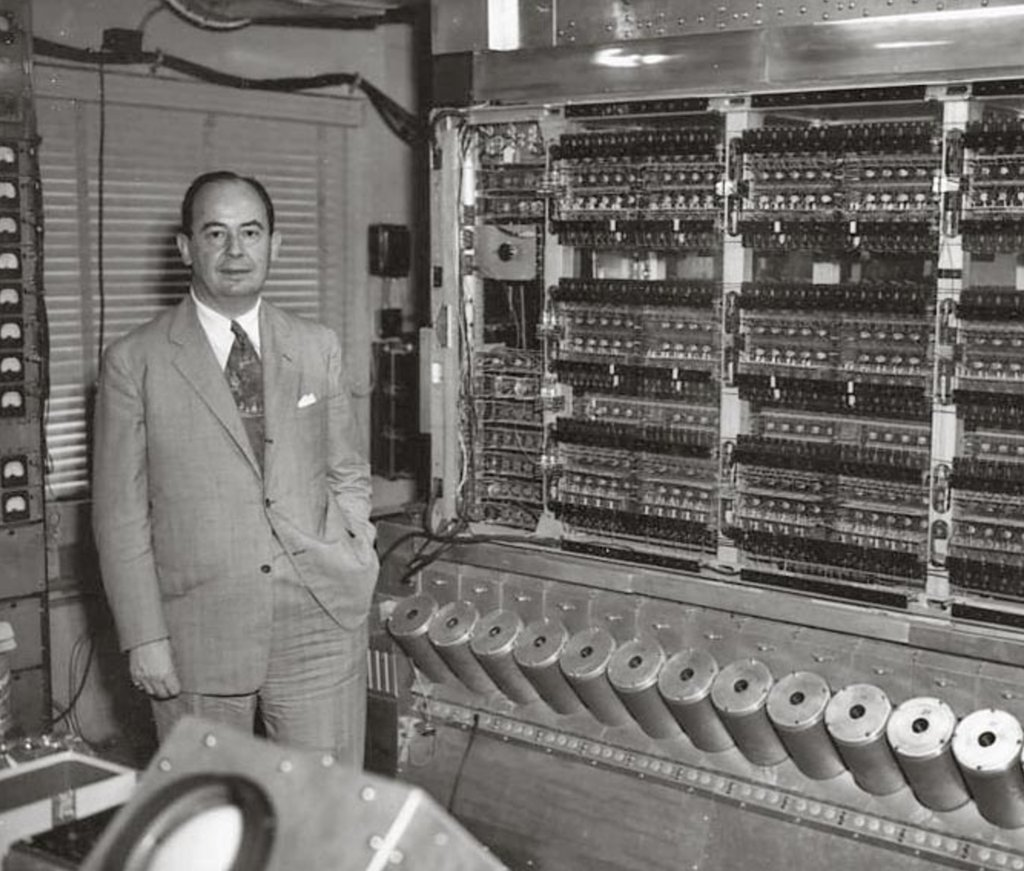
\includegraphics[width=11.5cm]{../resources/jpg/2.2.set.operations/neumann.jpg}
    \caption*{John Von Neumann in Turing's Cathedral.}
\end{figure}
\vspace{-1\baselineskip}
\subsection[Gamma is pi.]
    {
        \color{section}Theorem 61 \color{black} : gamma is pi.
    }
\documentclass[preview]{standalone}
\usepackage{amssymb, amsthm}
\usepackage{mathtools}
\usepackage{bm}


\newtheorem{theorem}{Theorem}
\renewcommand\qedsymbol{$\blacksquare$}


\begin{document}


\begin{theorem}[\textbf{2241}]
    Let \bm{$\Gamma$}, \bm{$\Pi$}, and \bm{$\Xi$} be sets.
    \begin{equation*}
        \bm{ \text{If }
            \Gamma \oplus \Xi 
                = 
            \Pi \oplus \Xi
                \text{, then } 
            \Gamma = \Pi
        }    
    \end{equation*}
\end{theorem}
\begin{proof} 
By contraposition. Note that the statement 
\bm{$
    \Gamma \oplus \Xi 
        = 
    \Pi \oplus \Xi
$}
is by definition 
\begin{equation*}
    \Big \langle \Gamma \cap \overline{\Xi} \Big \rangle 
        \cup 
    \Big \langle \overline{\Gamma} \cap \Xi \Big \rangle 
        \equiv
    \Big \langle \Pi \cap \overline{\Xi} \Big \rangle 
        \cup 
    \Big \langle \overline{\Pi} \cap \Xi \Big \rangle
\end{equation*}
Assume there exists an element \bm{$\zeta$} 
such that \bm{$\zeta \in \Gamma$} and \bm{$\zeta \notin \Pi$}. 
Thus, \bm{$\Gamma \nsubseteq \Pi$},
the negation of the consequent, by the definiton of subsets. 
By that hypothesis, 
\bm{$\zeta$} has to be in 
\bm{$\Gamma \cap \overline{\Xi}$} 
and cannot be in 
\bm{$\overline{\Gamma} \cap \Xi$}. 
This means that \bm{$\zeta$} is not in \bm{$\Xi$}. 
Neither can \bm{$\zeta$} be in 
\bm{$\Pi \cap \overline{\Xi}$}. 
And since \bm{$\zeta \notin \Xi$}, 
\bm{$\zeta$} cannot be in \bm{$\overline{\Pi} \cap \Xi$}. 
So \bm{$\zeta$} is in \bm{$\Gamma \oplus \Xi$} 
but not \bm{$\Pi \oplus \Xi$}. 
Therefore, 
\bm{$\Gamma \oplus \Xi \nsubseteq \Pi \oplus \Xi$},
by the definition of subsets.
The implication,
\begin{equation*}
    \Big \langle \Pi \not \subseteq \Gamma \Big \rangle
        \rightarrow
    \bigg[
        \Big \langle \Pi \oplus \Xi \Big \rangle
            \not \subseteq 
        \Big \langle \Gamma \oplus \Xi \Big \rangle
    \bigg]
\end{equation*} 
follows without loss of generality
$\therefore \text{\space} \bm{
    \Gamma \neq \Pi}$ 
implies 
\bm{$\Gamma \oplus \Xi \neq \Pi \oplus \Xi
}$.
\end{proof}


\end{document}
\pagebreak


\section{Lemmas}
\begin{figure}[!h]
    \centering
    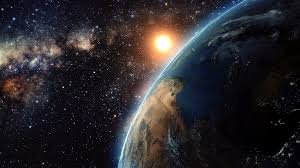
\includegraphics[width=14cm]{../resources/jpg/2.2.set.operations/sun.jpg}
\end{figure}


% =============================== 0001 Lemma 2201 =================================
\subsection[Lemma 1]{\color{section}Lemma 1}
\documentclass[preview]{standalone}
\usepackage{amssymb, amsthm}
\usepackage{mathtools}
\usepackage{bm}


\newtheorem{lemma}{Lemma}
\renewcommand\qedsymbol{$\blacksquare$}


\begin{document}


\begin{lemma}%[\textbf{2201}]
    Let \bm{$\mathrm{A}$}, and \bm{$\Lambda$} be sets.
    \begin{equation*}
        \bm{
            \mathrm{A} \oplus \Lambda
                =
            \Big \langle \mathrm{A} \cup \Lambda \Big \rangle
                \cap
            \Big \langle 
                \overline{\mathrm{A}} 
                    \cup 
                \overline{\Lambda} 
            \Big \rangle
        }
    \end{equation*}
\end{lemma}
\begin{proof}
    By Theorem 52,
    \bm{$
        \big \langle \mathrm{A} \oplus \Lambda \big \rangle
            \equiv
        \big \langle \mathrm{A} \cup \Lambda \big \rangle
            -
        \big \langle \mathrm{A} \cap \Lambda \big \rangle
    $}, 
    and by Theorem 45, that is
    \bm{$
        \big \langle \mathrm{A} \cup \Lambda \big \rangle
            \cap
        \big \langle \overline{\mathrm{A} \cap \Lambda} \big \rangle
    $}.
    By Demorgans law for the complement of set intersection,
    \begin{equation*}
        \Big \langle \mathrm{A} \cup \Lambda \Big \rangle
            \cap
        \Big \langle \overline{\mathrm{A} \cap \Lambda} \Big \rangle
            \equiv
        \Big \langle \mathrm{A} \cup \Lambda \Big \rangle
            \cap
        \Big \langle \overline{\mathrm{A}} \cup \overline{\Lambda} \Big \rangle
    \end{equation*}
    $\therefore \text{\space} \bm{
    \mathrm{A} \oplus \Lambda
        =
    \big \langle \mathrm{A} \cup \Lambda \big \rangle
        \cap
    \big \langle 
        \overline{\mathrm{A}} 
            \cup 
        \overline{\Lambda} 
    \big \rangle}$
\end{proof}


\end{document}
\vspace{2\baselineskip}
\sep
\pagebreak


% =============================== 0002 Lemma 2202 =================================
\subsection[Lemma 2]{\color{section}Lemma 2}
\documentclass[preview]{standalone}
\usepackage{amssymb, amsthm}
\usepackage{mathtools}
\usepackage{bm}


\newtheorem{lemma}{Lemma}
\renewcommand\qedsymbol{$\blacksquare$}


\begin{document}


\begin{lemma} %[\textbf{2202}]
    Let \bm{$\mathrm{A}$}, and \bm{$\Lambda$} be sets.
    \begin{equation*}
        \bm{
            \bigg[
                \Big \langle \mathrm{A} \cup \Lambda \Big \rangle
                    \cap
                \Big \langle 
                    \overline{\mathrm{A}} 
                        \cup 
                    \overline{\Lambda} 
                \Big \rangle
            \bigg]
                \cup
            \Lambda
                =
            \mathrm{A} \cup \Lambda
        }
    \end{equation*}
\end{lemma}
\begin{proof}
    Let \bm{$\Omega$} be the universe.
    By the law of distribution for set union over intersection,
    and by the associative law for set union,
    \begin{equation*}
        \bigg[
            \Big \langle \mathrm{A} \cup \Lambda \Big \rangle
                \cap
            \Big \langle 
                \overline{\mathrm{A}} 
                    \cup 
                \overline{\Lambda} 
            \Big \rangle
        \Big]
            \cup
        \Lambda
            \equiv
        \Big \langle \mathrm{A} \cup \Lambda \cup \Lambda \Big \rangle
            \cap
        \Big \langle 
            \overline{\mathrm{A}} 
                \cup 
            \overline{\Lambda} 
                \cup
            \Lambda
        \Big \rangle
    \end{equation*}
    By the idempotent law for set union, 
    and by the complement law for set union, that is
    \begin{equation*}
        \Big \langle \mathrm{A} \cup \Lambda \Big \rangle
            \cap
        \Big \langle 
            \overline{\mathrm{A}} 
                \cup 
            \Omega
        \Big \rangle
    \end{equation*}
    The right-hand side of this intersection is dominated by the universe,
    according to the domination law for set union. Thus, that is
    \bm{$\mathrm{A} \cup \Lambda$} intersect \bm{$\Omega$}.
    $\therefore \text{\space} \bm{
    \big[
        \big \langle \mathrm{A} \cup \Lambda \big \rangle
            \cap
        \big \langle 
            \overline{\mathrm{A}} 
                \cup 
            \overline{\Lambda} 
        \big \rangle
    \big]
        \cup
    \Lambda
        =
    \mathrm{A} \cup \Lambda
    }$, by the identity law for the intersection of sets.
\end{proof}


\end{document}
\begin{figure}[!h]
    \centering
    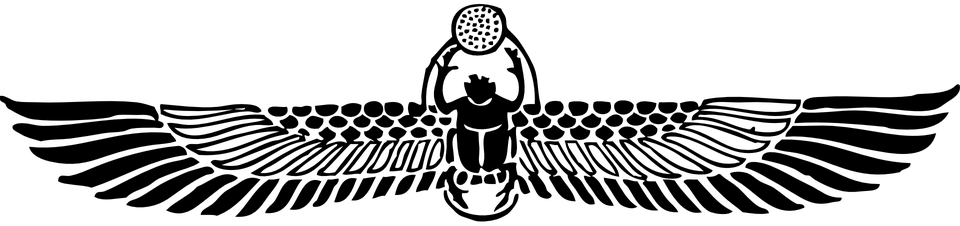
\includegraphics[width=8cm]{../resources/jpg/2.2.set.operations/scarab.png}
\end{figure}


% =============================== 0003 Lemma 2203 =================================
\subsection[Lemma 3]{\color{section}Lemma 3}
\documentclass[preview]{standalone}
\usepackage{amssymb, amsthm}
\usepackage{mathtools}
\usepackage{bm}


\newtheorem{lemma}{Lemma}
\renewcommand\qedsymbol{$\blacksquare$}


\begin{document}


\begin{lemma} %[\textbf{2203}]
    Let \bm{$\mathrm{A}$}, and \bm{$\Lambda$} be sets.
    \begin{equation*}
        \bm{
            \Big \langle \mathrm{A} \cup \Lambda \Big \rangle
                \cap
            \Big \langle 
                \overline{\mathrm{A}} 
                    \cup 
                \overline{\Lambda} 
            \Big \rangle
                \cap
            \Lambda
                =
            \Lambda \cap \overline{\mathrm{A}}
        }
    \end{equation*}
\end{lemma}
\begin{proof}
    By the law of distribution for set intersection over set union,
    \begin{equation*}
        \Big \langle \mathrm{A} \cup \Lambda \Big \rangle
            \cap
        \Big \langle 
            \overline{\mathrm{A}} 
                \cup 
            \overline{\Lambda} 
        \Big \rangle
            \cap
        \Lambda
            =
        \Big \langle \mathrm{A} \cup \Lambda \Big \rangle
            \cap
        \bigg[
            \Big \langle \overline{\mathrm{A}} \cap \Lambda \Big \rangle
                \cup
            \Big \langle \overline{\Lambda} \cap \Lambda \Big \rangle
        \bigg]
    \end{equation*}
    \bm{$\overline{\Lambda} \cap \Lambda \equiv \varnothing$}, 
    by the complement law for set intersection. 
    Therefore, the term in the brackets is \bm{$\overline{\mathrm{A}} \cap \Lambda$},
    by the identity law for set union. By the associative law for set intersection, what we have left is
    \begin{equation*}
        \Big \langle \mathrm{A} \cup \Lambda \Big \rangle
            \cap
        \overline{\mathrm{A}}
            \cap
        \Lambda
    \end{equation*}
    \bm{$\mathrm{A} \cup \Lambda$} is absorbed by \bm{$\Lambda$}, 
    by the absorption laws for sets, 
    since sets are commutative over intersection, 
    by the commutative law for set intersection.
    $\therefore \text{} \bm{
        \big \langle \mathrm{A} \cup \Lambda \big \rangle
            \cap
        \big \langle 
            \overline{\mathrm{A}} 
                \cup 
            \overline{\Lambda} 
        \big \rangle
            \cap
        \Lambda
            =
        \Lambda \cap \overline{\mathrm{A}}
    }$. 
\end{proof}


\end{document}
\pagebreak


% =============================== 0004 Lemma 2204 =================================
\subsection[Lemma 4]{\color{section}Lemma 4}
\documentclass[preview]{standalone}
\usepackage{amssymb, amsthm}
\usepackage{mathtools}
\usepackage{bm}


\newtheorem{lemma}{Lemma}
\renewcommand\qedsymbol{$\blacksquare$}


\begin{document}


\begin{lemma} %[\textbf{2204}]
    Let \bm{$\Gamma$}, \bm{$\Pi$}, and \bm{$\Xi$} be sets.
    \begin{equation*}
    \bm{
        \Big \langle \Gamma \cup \Pi \Big \rangle
            \cap
        \Big \langle \overline{\Gamma} \cup \overline{\Pi} \Big \rangle
            \cap
        \overline{\Xi}
            =
        \Big \langle \Pi \cap \overline{\Gamma} \cap \overline{\Xi} \Big \rangle
            \cup
        \Big \langle \Gamma \cap \overline{\Pi} \cap \overline{\Xi} \Big \rangle
        }
    \end{equation*}
\end{lemma}
\begin{proof}
    Distributing the term \bm{$\Gamma \cup \Pi$} over the union of 
    \bm{$\overline{\Gamma}$} and \bm{$\overline{\Pi}$},
    by the law of distribution for the intersection of sets over union,
    in the left-hand side of the equation expressed by the lemma is
    \begin{equation*}
        \bigg[
            \Big \langle \Gamma \cup \Pi \Big \rangle
                \cap
            \overline{\Gamma}
        \bigg]
            \cup
        \bigg[
            \Big \langle \Gamma \cup \Pi \Big \rangle
                \cap
            \overline{\Pi}
        \bigg]
            \cap
        \overline{\Xi}
    \end{equation*}
    Again, by the law of distribution for intersection over set union,
    \begin{equation*}
        \equiv
        \bigg[
            \Big \langle \Gamma \cap \overline{\Gamma} \Big \rangle
                \cup
            \Big \langle \Pi \cap \overline{\Gamma} \Big \rangle
        \bigg]
            \cup
        \bigg[
            \Big \langle \Gamma \cap \overline{\Pi} \Big \rangle
                \cup
            \Big \langle \Pi \cap \overline{\Pi} \Big \rangle
        \bigg]
            \cap
        \overline{\Xi}
    \end{equation*}
    \bm{$\Gamma \cap \overline{\Gamma}$} and \bm{$\Pi \cap \overline{\Pi}$}
    are both empty, by the domination law for set intersection. And any set,
    union the empty set, is itself, by the identity law for set union. Thus,
    by association, what is left is
    \begin{equation*}       
        \bigg[
            \Big \langle \Pi \cap \overline{\Gamma} \Big \rangle
                \cup
            \Big \langle \Gamma \cap \overline{\Pi} \Big \rangle
        \bigg]
            \cap
        \overline{\Xi}
    \end{equation*}
    $\therefore \bm{
        \big \langle \Gamma \cup \Pi \big \rangle
            \cap
        \big \langle \overline{\Gamma} \cup \overline{\Pi} \big \rangle
            \cap
        \overline{\Xi}
            =
        \big \langle \Pi \cap \overline{\Gamma} \cap \overline{\Xi} \big \rangle
            \cup
        \big \langle \Gamma \cap \overline{\Pi} \cap \overline{\Xi} \big \rangle
    }$,
    by the law of distribution for set intersection over set union,
    and by association for the intersection of sets.
\end{proof}


\end{document}
\sep
\vspace{1.5\baselineskip}
\begin{figure}[!h]
    \centering
    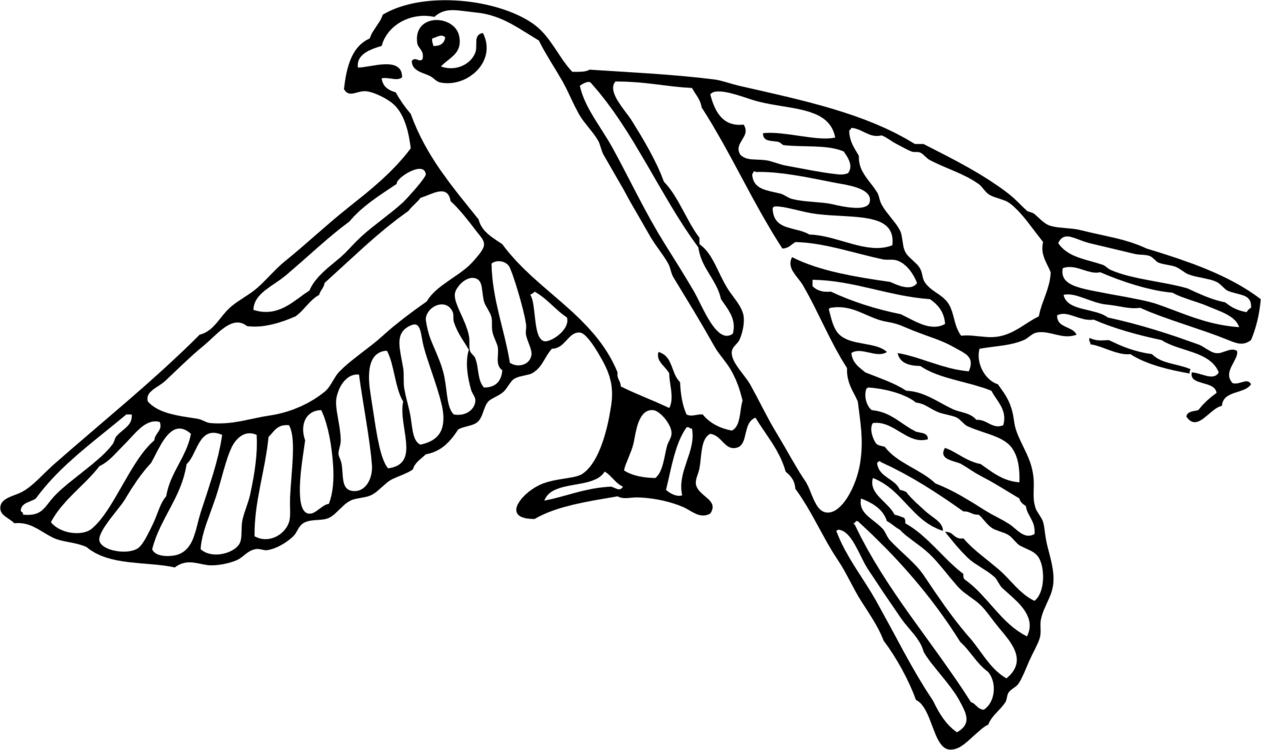
\includegraphics[width=8cm]{../resources/jpg/2.2.set.operations/bird.png}
\end{figure}
\pagebreak



% =============================== 0005 Lemma 2205 =================================
\subsection[Lemma 5]{\color{section}Lemma 5}
\documentclass[preview]{standalone}
\usepackage{amssymb, amsthm}
\usepackage{mathtools}
\usepackage{bm}


\newtheorem{lemma}{Lemma}
\renewcommand\qedsymbol{$\blacksquare$}


\begin{document}


\begin{lemma} %[\textbf{2205}]
    Let \bm{$\Gamma$}, \bm{$\Pi$}, and \bm{$\Xi$} be sets.
    \begin{equation*}
        \bm{
            \overline{
                \Big \langle \Gamma \cup \Pi \Big \rangle
                    \cap
                \Big \langle \overline{\Gamma} \cup \overline{\Pi} \Big \rangle
            }
                \cap
            \Xi
                    =
            \Big \langle \overline{\Gamma} \cap \overline{\Pi} \cap \Xi \Big \rangle
                \cup
            \Big \langle \Gamma \cap \Pi \cap \Xi \Big \rangle
        }
    \end{equation*}
\end{lemma}
\begin{proof}
    By DeMorgans Law for sets, 
    the expression occurring in the left-hand side of the equation in the lemma is
    \begin{equation*}
        \bigg[
            \Big \langle \overline{\Gamma \cup \Pi} \Big \rangle
                \cup
            \Big \langle \overline{\overline{\Gamma} \cup \overline{\Pi}} \Big \rangle
        \bigg]
            \cap
        \Xi
    \end{equation*}
    Which, again by DeMorgans law for sets, and by the complementation law for sets, is equivalent to
    \begin{equation*}
        \bigg[
            \Big \langle \overline{\Gamma} \cap \overline{\Pi} \Big \rangle
                \cup
            \Big \langle \Gamma \cap \Pi \Big \rangle
        \bigg]
            \cap
        \Xi
    \end{equation*}
    By the distributive law for set intersection over set union,
    and by associative law for the intersection of sets, that is
    \begin{equation*}
        \Big \langle \overline{\Gamma} \cap \overline{\Pi} \cap \Xi \Big \rangle
            \cup
        \Big \langle \Gamma \cap \Pi \cap \Xi \Big \rangle
    \end{equation*}
    $\therefore \bm{
        \overline{
            \big \langle \Gamma \cup \Pi \big \rangle
                \cap
            \big \langle \overline{\Gamma} \cup \overline{\Pi} \big \rangle
        }
            \cap
        \Xi
            =
        \big \langle \overline{\Gamma} \cap \overline{\Pi} \cap \Xi \big \rangle
            \cup
        \big \langle \Gamma \cap \Pi \cap \Xi \big \rangle
    }$.
\end{proof}


\end{document}
\sep
\pagebreak


\end{document}